\documentclass[../../main/main.tex]{subfiles}
\graphicspath{{./figures/}}

\dominitoc
\faketableofcontents

\makeatletter
\renewcommand{\@chapapp}{M\'ecanique -- chapitre}
\makeatother

% \toggletrue{student}
% \HideSolutionstrue
% \toggletrue{corrige}
% \renewcommand{\mycol}{black}
\renewcommand{\mycol}{gray}

\begin{document}
\setcounter{chapter}{0}

\chapter{Cin\'ematique du point}

\vfill

\begin{prgm}
	\begin{tcb}*(ror)"know"{Savoirs}
		\begin{itemize}
			\item Espace et temps classiques. Notion de référentiel. Caractère relatif
			      du mouvement. Caractère absolu des distances et des intervalles de
			      temps.
			\item Citer une situation où la description classique de l'espace ou du
			      temps est prise en défaut.

			\item Identifier les degrés de liberté d'un mouvement. Choisir un système
			      de coordonnées adapté au problème.
		\end{itemize}
	\end{tcb}
	\begin{tcb}*(ror)"how"{Savoir-faire}
		\begin{itemize}
			\item Coordonnées cartésiennes~: exprimer à partir d'un schéma le
			      déplacement élémentaire, construire le trièdre local associé et en
			      déduire géométriquement les composantes du vecteur vitesse.

			\item Établir les expressions des composantes des vecteurs position,
			      déplacement élémentaire, vitesse et accélération en coordonnées
			      cartésiennes.

			\item Mouvement à vecteur accélération constant~: exprimer le vecteur
			      vitesse et le vecteur position en fonction du temps. Établir
			      l'expression de la trajectoire en coordonnées cartésiennes.

			\item Situer qualitativement la direction du vecteur vitesse et du
			      vecteur accélération pour une trajectoire plane.
		\end{itemize}
	\end{tcb}
\end{prgm}

\vfill

% \newpage

% \vspace*{\fill}
\vfill
\minitoc
\vfill
% \vspace*{\fill}

\newpage

\begin{pycode}
	import numpy as np
	c = 299753458 # m.s^-1
	v = 0.9997*c  # m.s^-1
	tau = 2.197e-6 # s
	d_nr = v*tau
	gamma = 1/np.sqrt(1 - v**2/c**2)
	tau_p = gamma*tau
	d_r = v*tau_p
\end{pycode}

La \textbf{cinématique} est l'étude du mouvement en soi. On ne s'intéresse pas
aux causes qui ont donné naissance au mouvement. Avant toute chose, introduisons
le vocabulaire autour de l'objet d'étude.

\section{Système et point matériel}
\subsection{Système}
\begin{tcb*}(defi){Système}
	En mécanique, le \textbf{système} est l'objet ou groupe
	d'objets dont on souhaite étudier le mouvement.
\end{tcb*}

La définition du système est \textbf{primordiale et indispensable} pour la
mécanique. En effet, l'étude du mouvement sera radicalement différente entre les
systèmes \{bille\} et \{bille+Terre\}. Il en sera de même en dynamique, où ce
sont les forces \textbf{extérieures} au système qui entrent en jeu, il faut donc
définir l'extérieur.

\subsection{Point matériel}

Dans la cadre de la mécanique du point, la forme de l'objet importe peu. Ainsi,
on choisira de suivre un point caractéristique du système, souvent son centre de
gravité. Celui-ci pourra être repéré dans l'espace et le temps par 3+1
coordonnées.

\begin{tcb*}(defi){Point matériel}
	\psw{
		Le point matériel est le point qui représente l'objet auquel on affecte
		toute la masse de l'objet considéré. Ce point, appelé souvent M et affecté
		de la masse $m$, est le point géométrique que l'on repère dans l'espace pour
		connaître son mouvement.}%\vspace{-10pt}
\end{tcb*}

\section{Description et paramétrage du mouvement}
\subsection{Notion de référentiel et relativité du mouvement}

Pour décrire le mouvement d'un objet, on doit~:
\begin{itemize}
	\item dire par \underline{rapport à quoi} il se déplace~: on définit alors
	      une \textbf{origine}~;
	\item dire dans \underline{quelle direction} il se déplace~: on fixe alors
	      un \textbf{repère} (système de coordonnées)~;
	\item dire sur \underline{quel intervalle de temps} il se déplace~: on
	      définit un repère de temps.
\end{itemize}

\begin{tcb*}(defi){Référentiel}
	Un \textbf{référentiel}, noté $\Rc$, est une référence permettant de décrire
	le mouvement d'un objet, constitué par~:
	\psw{
		\begin{itemize}
			\item un repère permettant de décrire l'espace~;
			\item une horloge permettant de mesurer le temps.
		\end{itemize}
	}%\vspace{-10pt}
\end{tcb*}

Un mouvement est toujours relatif, et \textbf{la description d'un mouvement
	dépend du référentiel}. Ainsi, on notera les grandeurs liées à un référentiel
\textit{via} l'indication de celui-ci en indice, précédé d'une barre oblique ou
verticale selon la taille de la grandeur~:
\[  \boxed{\vv{x}_{/\Rc}}
	\qou
	\boxed{\eval{\dv{\vv{x}}{t}}_{\Rc}}\]

\begin{tcb*}(exem)<lfnt>'l'{Mouvement relatif}
	\begin{itemize}
		\item Du point de vue de san voisin-e, læ passagær d'un train est
		      immobile. Du point de vue du quai, cælui-ci est en translation.
		\item Du point de vue d'um cycliste, la valve de la roue est en rotation
		      autour de l'axe de la roue. Selon um passant-e immobile, elle suit
		      un mouvement de cycloïde. Son altitude atteint $0$ à chaque tour de
		      roue.
		      \begin{center}
			      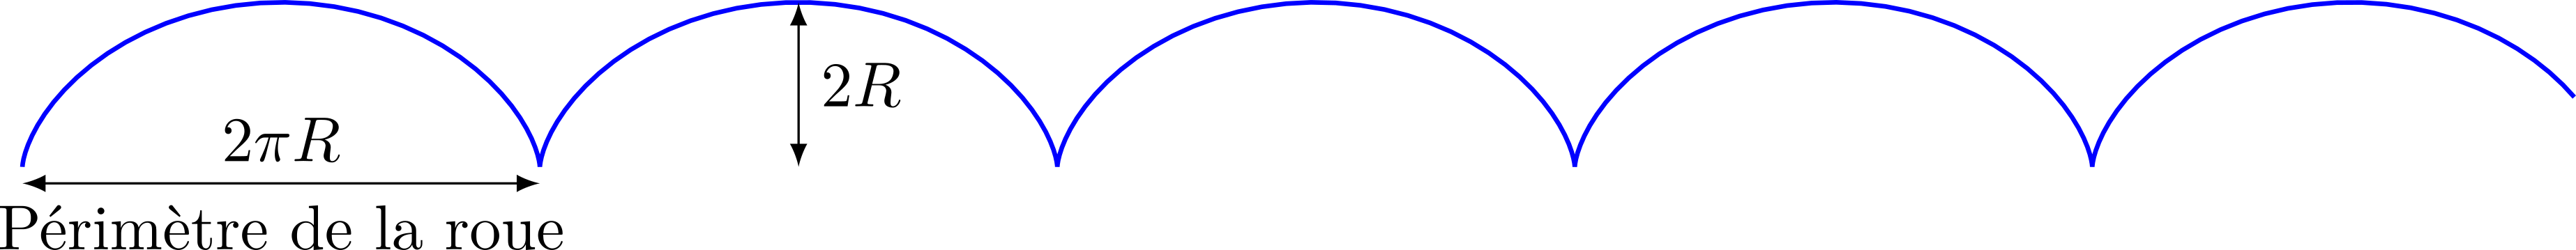
\includegraphics[width=\linewidth]{roue}
		      \end{center}
	\end{itemize}
\end{tcb*}

\begin{tcb*}(rema){Mécanique relativiste}
	Nous resterons ici en mécanique \textbf{classique}, c'est-à-dire que les
	corps étudiés auront une vitesse très inférieure à celle de la lumière dans
	le vide. Ce faisant, les mesures de longueurs ou de durées seront
	\textbf{absolues} et indépendantes du référentiel. Ça n'est pas le cas en
	mécanique \textit{relativiste}.
	\bigbreak
	Par exemple, les muons sont des particules très instables, produites par le
	rayonnement cosmique dans la haute atmosphère. Ils se désintègrent normalement
	au bout de $\tau\ind{labo} = \py{fr'\SI{{{tau:.2e}}}{{s}}'}$. Leur vitesse est
	mesurée à $v\ind{muon} \approx \num{0.9997}c$.
	\smallbreak
	On s'attendrait donc à ce que de sa formation en altitude à sa désintégration
	vers le sol, un muon parcourt $d\ind{NR} = v\ind{muon} \times \tau\ind{labo} =
		\py{fr'\SI{{{d_nr:.2f}}}{{m}}'}$, et qu'il n'y en ait presque aucun à la
	surface terrestre.
	\smallbreak
	En réalité, on en détecte énormément au sol et même sous la mer~! En mécanique
	classique, cela reviendrait à leur attribuer une vitesse de plusieurs millions
	de kilomètres par seconde. La théorie de la relativité nous expliquant que la
	vitesse de la lumière est indépassable, ceci paraît absurde. C'est notre
	manière d'interpréter les mesures qui s'avère fausse~: le temps de vie d'un
	muon \textit{mesuré sur Terre} n'est pas le même que son \textit{temps
		propre}. On obtient
	\[
		\tau\ind{propre} = \gamma\tau\ind{labo}
		\qav
		\gamma = \frac{1}{\sqrt{1-\frac{v^{2}}{c^{2}}}}
	\]
	et ici, $\gamma = \py{fr'\num{{{gamma:.2e}}}'}$. Par dilatation du temps, le
	muon parcourt une plus grand distance en gardant la même vitesse, ici jusqu'à
	\[
		d\ind{R} = \py{fr'\SI{{{d_r:.2e}}}{{m}}'}
	\]
\end{tcb*}
\subsection{Exemples de référentiels}

Le mouvement dépendant du référentiel, il faut choisir le référentiel adéquat
par rapport au mouvement que l'on souhaite étudier. Souvent, on choisit parmi
trois référentiels classiques~:

\begin{itemize}

	\item Le référentiel \textbf{héliocentrique} est un référentiel dont le
	      centre du repère est situé au centre du \textbf{Soleil}, et les trois
	      axes du repère sont dirigés vers \textbf{trois étoiles lointaines
		      considérées comme fixes}~; il est utile pour étudier les mouvements des
	      planètes du système solaire.

	\item Le référentiel \textbf{géocentrique} est un référentiel centré au
	      centre de la \textbf{Terre}, ses trois axes sont dirigés vers les trois
	      \textbf{mêmes étoiles} que celles du référentiel de héliocentrique; il
	      est utilise pour étudier les mouvements de satellites terrestres par
	      exemple ;

	\item Les référentiels \textbf{terrestres} sont des référentiels liés à des
	      objets fixes à la \textbf{surface} de la Terre~: lui est souvent associé
	      un repère cartésien. Pour tous les mouvements qui se déroulent à la
	      surface de la Terre, ce référentiel est approprié.
\end{itemize}

\subsection{Vecteur, base de projection et repère}
Pour décrire le mouvement d'un point dans l'espace, il est nécessaire d'utiliser
des vecteurs.
\begin{tcb*}(defi){Vecteur}
	Un vecteur est un objet mathématique qui se dénote avec une flèche vers la
	droite au-dessus d'une lettre~: $\vec{\cdot}$, et ayant~:\smallbreak
	\begin{minipage}{0.40\linewidth}
		\begin{itemize}
			\item
			      \psw{
				      Un \textbf{point d'application}~;
			      }
			\item
			      \psw{
				      Une \textbf{direction}~;
			      }
		\end{itemize}
	\end{minipage}
	\begin{minipage}{0.50\linewidth}
		\begin{itemize}
			\item
			      \psw{
				      Un \textbf{sens}~;
			      }
			\item
			      \psw{
				      Une distance appelée \textbf{norme}, notée $\norm{\vec{\cdot}}$.
			      }
		\end{itemize}
	\end{minipage}
	\begin{framed}
		\centering
		\psw{
			\textbf{Une} égalité de vecteurs donne \textbf{trois} égalités de
			scalaires, pour chaque direction de l'espace.
		}
	\end{framed}
\end{tcb*}

On utilise pour ça une \textbf{base orthonormée directe}, constituée de 3
vecteurs~:

\noindent
\begin{minipage}{0.70\linewidth}
	\begin{itemize}
		\bitem{Ortho}~: les trois vecteurs de la base sont orthogonaux
		entre eux~;
		\bitem{Normée}~: la norme des trois vecteurs de la base est égale
		à 1. On dit qu'ils sont \textit{unitaires}~;
		\bitem{Directe}~: respecte la règle de la main droite (chaque
		vecteur est égal au produit vectoriel des deux précédents).
	\end{itemize}
\end{minipage}
\hfill
\begin{minipage}{0.20\linewidth}
	\begin{center}
		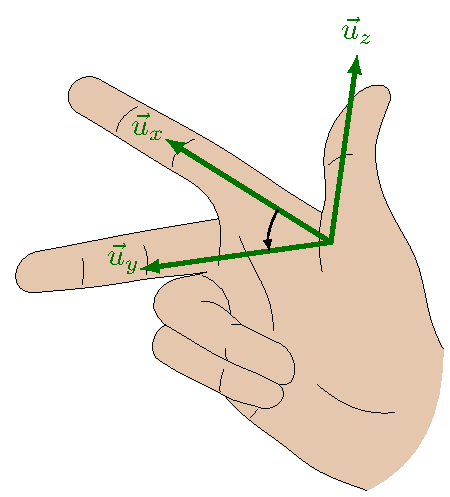
\includegraphics[width=\linewidth]{righthand}
	\end{center}
\end{minipage}
\hfill~

Ainsi pour une base générique $\left(\vv{i}, \vv{j}, \vv{k}\right)$, on
représente de manière équivalente un vecteur par ses composantes sur chaque
vecteur de base exprimées en colonne, ou par sa représentation explicite en
fonction desdits vecteurs de base~:
\[
	\vv{A} = \mqty(a_i\\a_j\\a_k)
	\Lra
	\vv{A} = a_i \vv{i} + a_j \vv{j} + a_k \vv{k}
\]

Les vecteurs de base n'ont \textbf{pas d'unité}. Ils définissent les trois
directions dans lesquelles le point M pourrait se mouvoir. Pour que le repérage
dans l'espace du point M soit complet, on ajoute une origine O à la base~:
l'ensemble d'une \textbf{base} et d'une \textbf{origine} constituent un
\textbf{repère}. Le plus simple est le repère cartésien~:
\begin{tcb*}[sidebyside, righthand ratio=.25](defi){Repère cartésien}
	\psw{
		Le repère cartésien est constitué d'une origine O autour de laquelle
		sont définis trois vecteurs $\ux$, $\uy$ et $\uz$ de \textbf{direction
			constante dans le temps}. On trouve parfois la notation $\ex$, $\ey$,
		$\ez$.}
	\bigbreak
	Jusqu'à notifié autrement, ce sera notre repère de prédilection.
	\tcblower
	\begin{center}
		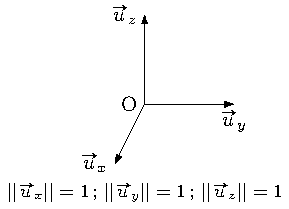
\includegraphics[width=\linewidth]{cart}
		\captionof{figure}{Repère cartésien.}
	\end{center}
\end{tcb*}

\begin{tcb*}[breakable](impo){Différence référentiel/repère}
	Il ne faut pas confondre le \textbf{référentiel}, c'est-à-dire le système de
	référence (notion \textit{physique}) avec le \textbf{repère}, c'est-à-dire
	l'outil géométrique qui sert à décrire le mouvement (notion
	\textit{mathématique}). Il y a une infinité de repères différents qui peuvent
	être associés à un même référentiel.
\end{tcb*}

\subsection{Projection d'un vecteur sur un autre}
Lors de l'étude de l'évolution d'un vecteur, il est commun de ne s'intéresser
qu'à certaines composantes dudit vecteur sur les vecteurs de base du repère
choisi. S'il est défini à partir ses composantes c'est une évidence, mais
souvent on aura des vecteurs définis par une \textbf{norme} et un \textbf{angle}
par rapport à l'un des axes.
\begin{tcb*}[sidebyside, righthand ratio=.4](tool){Projection vectorielle (2D)}
	Pour déterminer les coordonnées d'un vecteur sur les vecteurs de base d'un
	repère, on réalise une \textbf{projection}~:
	\psw{
		\[
			\vv{a}\!\cdot\!\!\ux = a_x
			\qet
			\vv{a}\!\cdot\!\!\uy = a_y
		\]
	}
	On peut alors utiliser les propriétés du produit scalaire~:
	\[
		\vv{a}\cdot \vv{b} = \norm{a}\norm{b}\cos(\theta)
	\]
	avec $\tt$ l'angle entre les vecteurs, pris \textbf{positivement en sens
		trigonométrique} (convention non explicite).
	\bigbreak
	On pourra également trouver les dépendances des composantes selon cosinus ou
	sinus par des tests de vraisemblance.
	\tcblower
	\begin{center}
		\sswitch{
			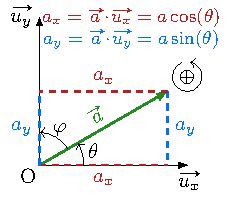
\includegraphics[width=\linewidth, draft=true]{proj}
		}{
			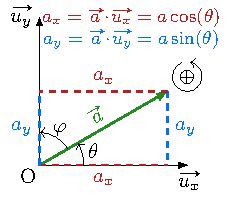
\includegraphics[width=\linewidth]{proj}
		}
		\vspace{-15pt}
		\captionof{figure}{Projection 2D}
	\end{center}
\end{tcb*}


\section{Position, vitesse et accélération}
\subsection{Position}
\subsubsection{Définition}

\begin{tcb*}[sidebyside, righthand ratio=.29](defi){Position en cartésiennes.}
	Le vecteur position noté $\OM(t)$ est le vecteur qui permet de repérer
	un point M d'un système dans l'espace et le temps par rapport à
	l'origine O d'un repère. \textbf{Il est homogène à une distance}.
	\smallbreak
	En coordonnées cartésiennes, la position d'un point M par rapport à
	l'origine O s'écrit~:
	\[\psw{\OM(t) = x(t)\ux + y(t)\uy + z(t)\uy}\]
	et sa \textbf{norme} se calcule avec~:
	\[\psw{\OMr = \norm{\OM} = \sqrt{x(t)^2 + y(t)^2 + z(t)^2}}\]
	\tcblower
	\begin{center}
		\sswitch{
			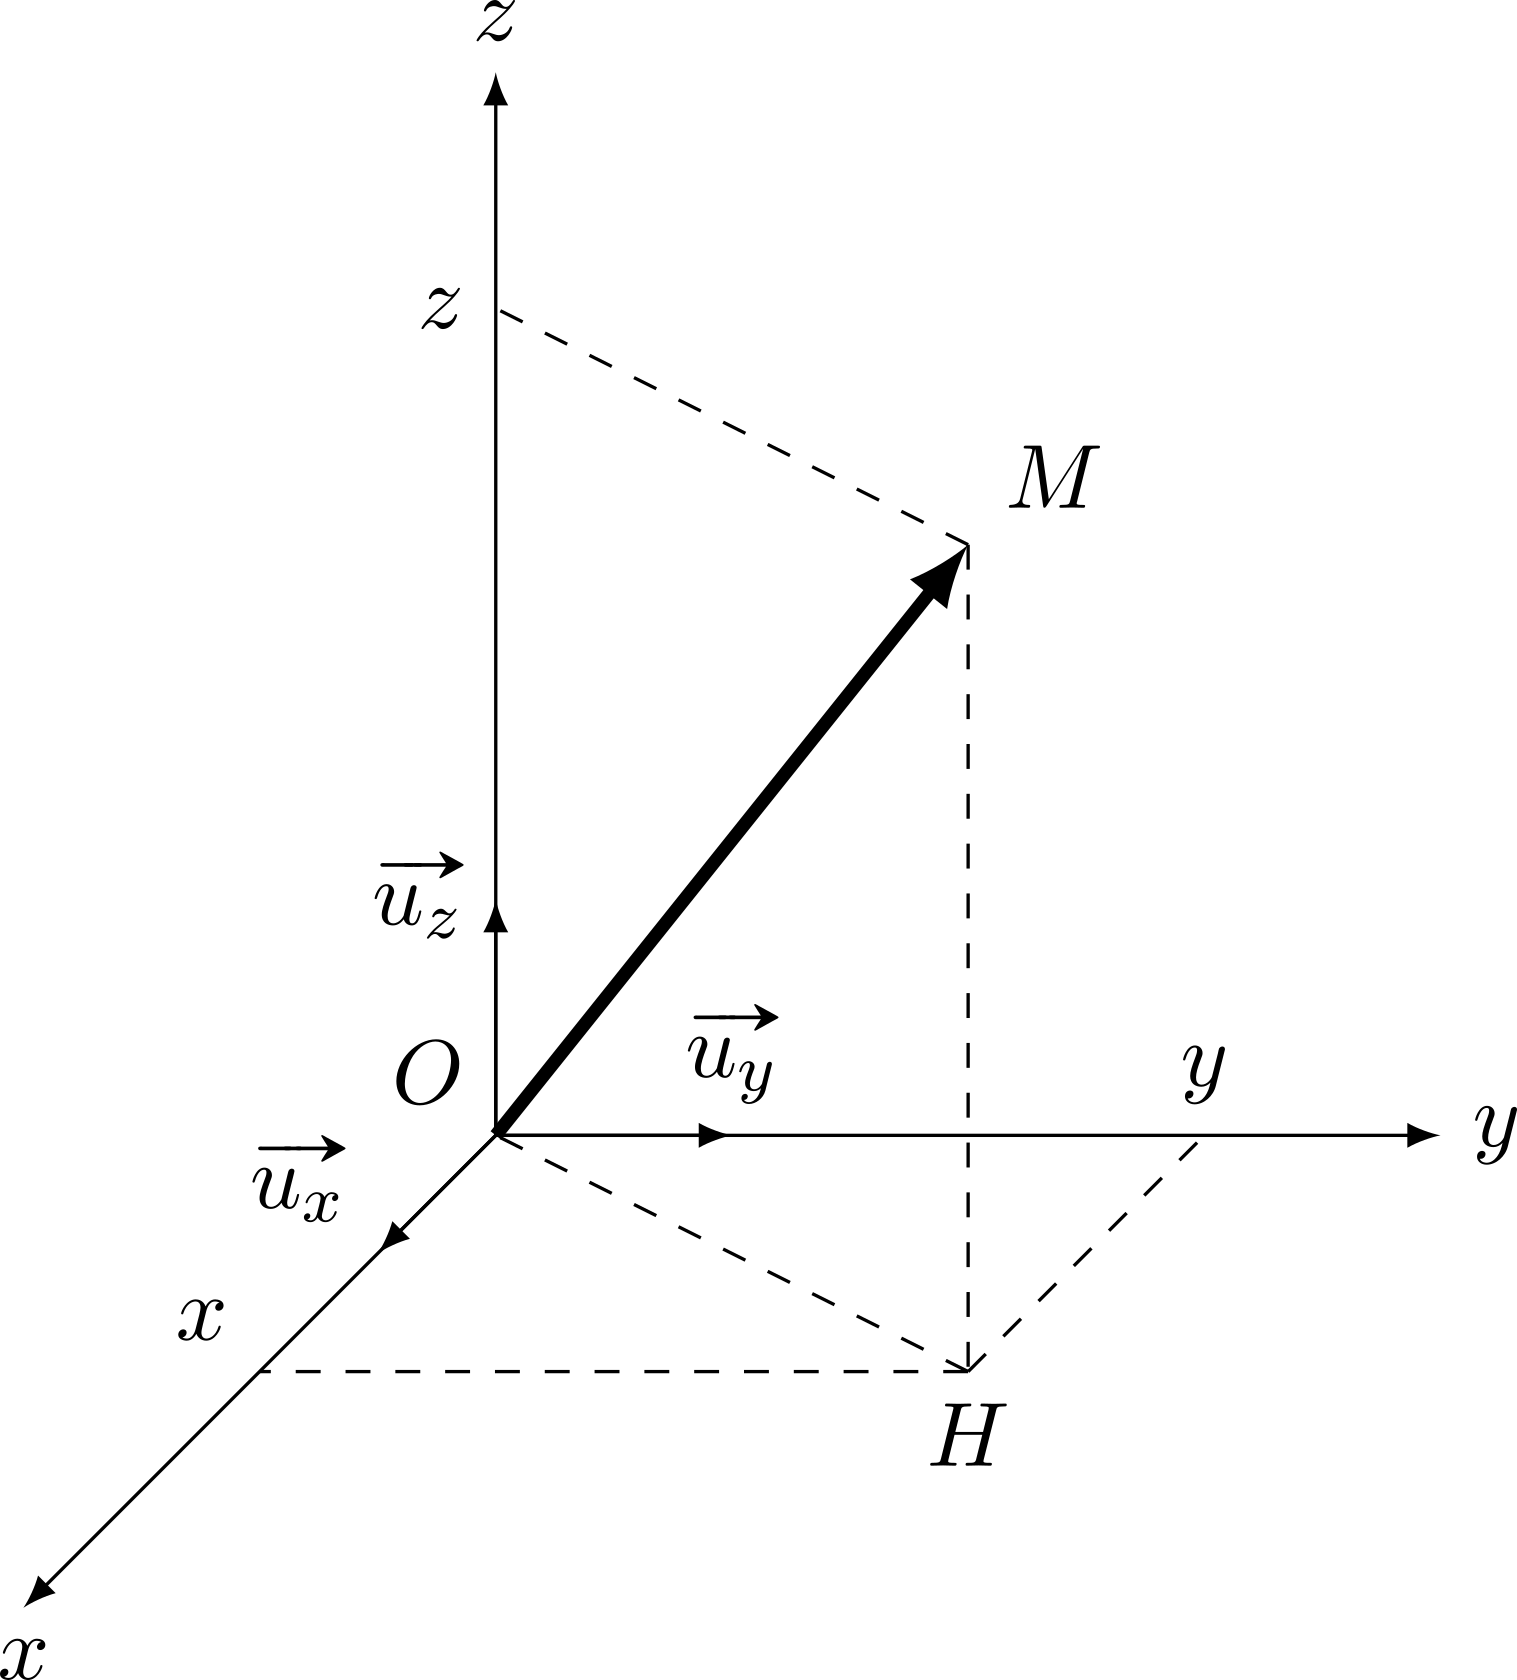
\includegraphics[width=\linewidth, draft=true]{vec_pos}
		}{
			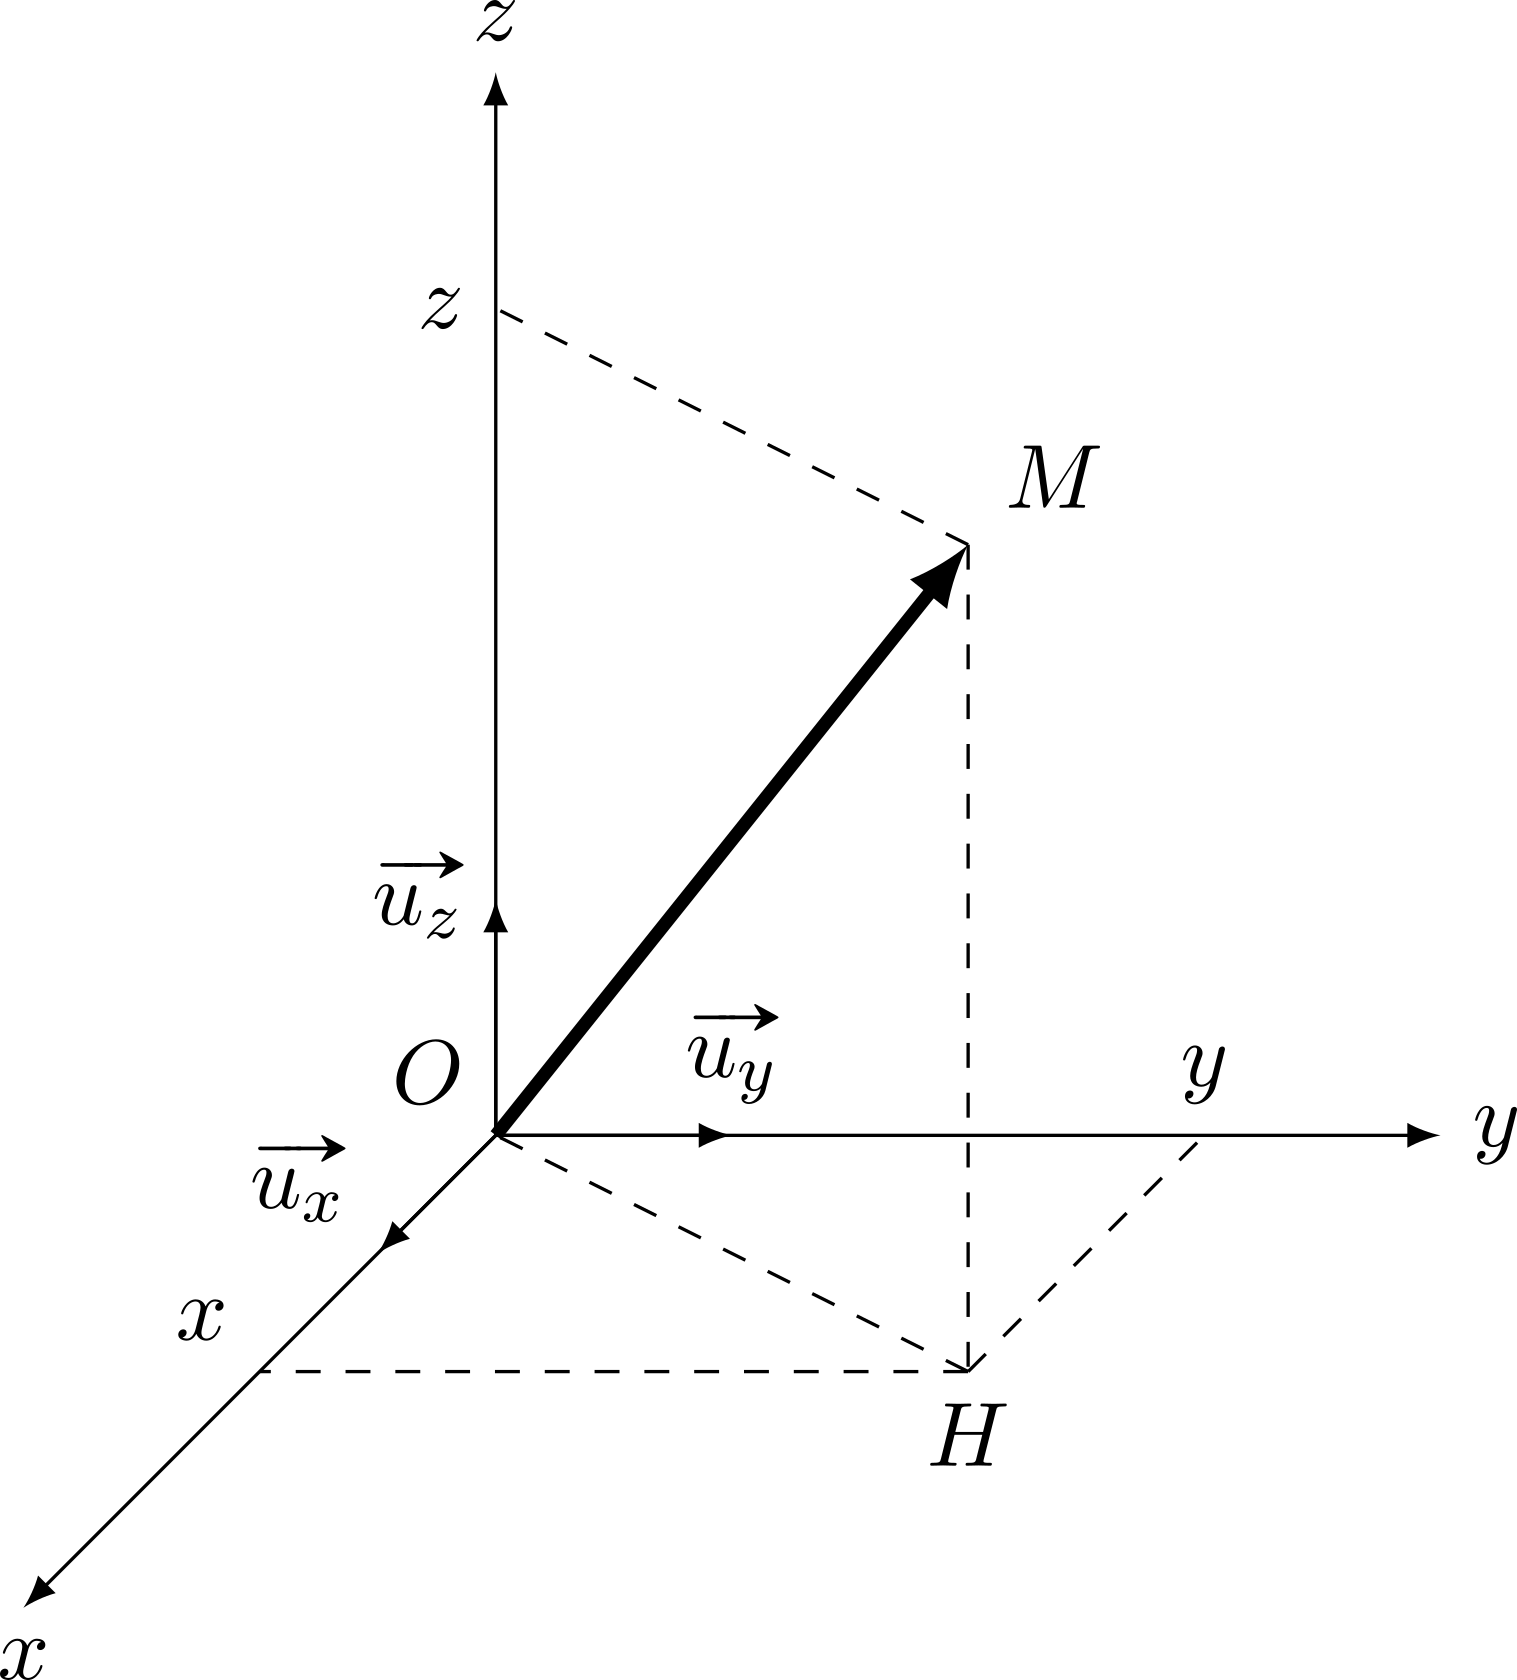
\includegraphics[width=\linewidth]{vec_pos}
		}
		\vspace{-15pt}
		\captionof{figure}{Position cartésienne.}
	\end{center}
\end{tcb*}

\subsubsection{Déplacement élémentaire}
\begin{tcb*}[sidebyside, righthand ratio=.25](defi){Déplacement élémentaire
			cartésien}
	Le \textbf{déplacement élémentaire} est le déplacement infiniment petit du
	point M pendant un temps infinitésimal $\dt$~:
	\[\psw{\dd\OM = \OM(t+\dt)-\OM(t)}\]
	En coordonnées cartésiennes,
	\[\psw{\boxed{\dd\OM = \dd{x}\ux + \dd{y}\uy + \dd{z}\uz}}\]
	\tcblower
	\begin{center}
		\sswitch{
			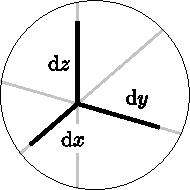
\includegraphics[width=\linewidth, draft=true]{delem_cart}
		}{
			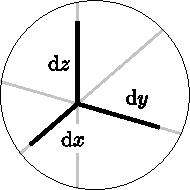
\includegraphics[width=\linewidth]{delem_cart}
		}
		\vspace{-15pt}
		\captionof{figure}{$\dd{\protect\OM}$ en cartésiennes.}
	\end{center}
\end{tcb*}

\subsubsection{Équations horaires et trajectoire}
\begin{tcb*}(defi)<lfnt>'l'{Équations horaires}
	Les \textbf{équations horaires} du mouvement sont les fonctions $x(t)$,
	$y(t)$ et $z(t)$ exprimées \textbf{explicitement} en fonction du temps $t$.
\end{tcb*}

En TP, on pourra étudier l'évolution de $x(t)$ et $y(t)$ dans différents cas~:
\bigbreak

\begin{minipage}{0.31\linewidth}
	\begin{itemize}
		\item chute dans le glycérol~:
	\end{itemize}
	\begin{center}
		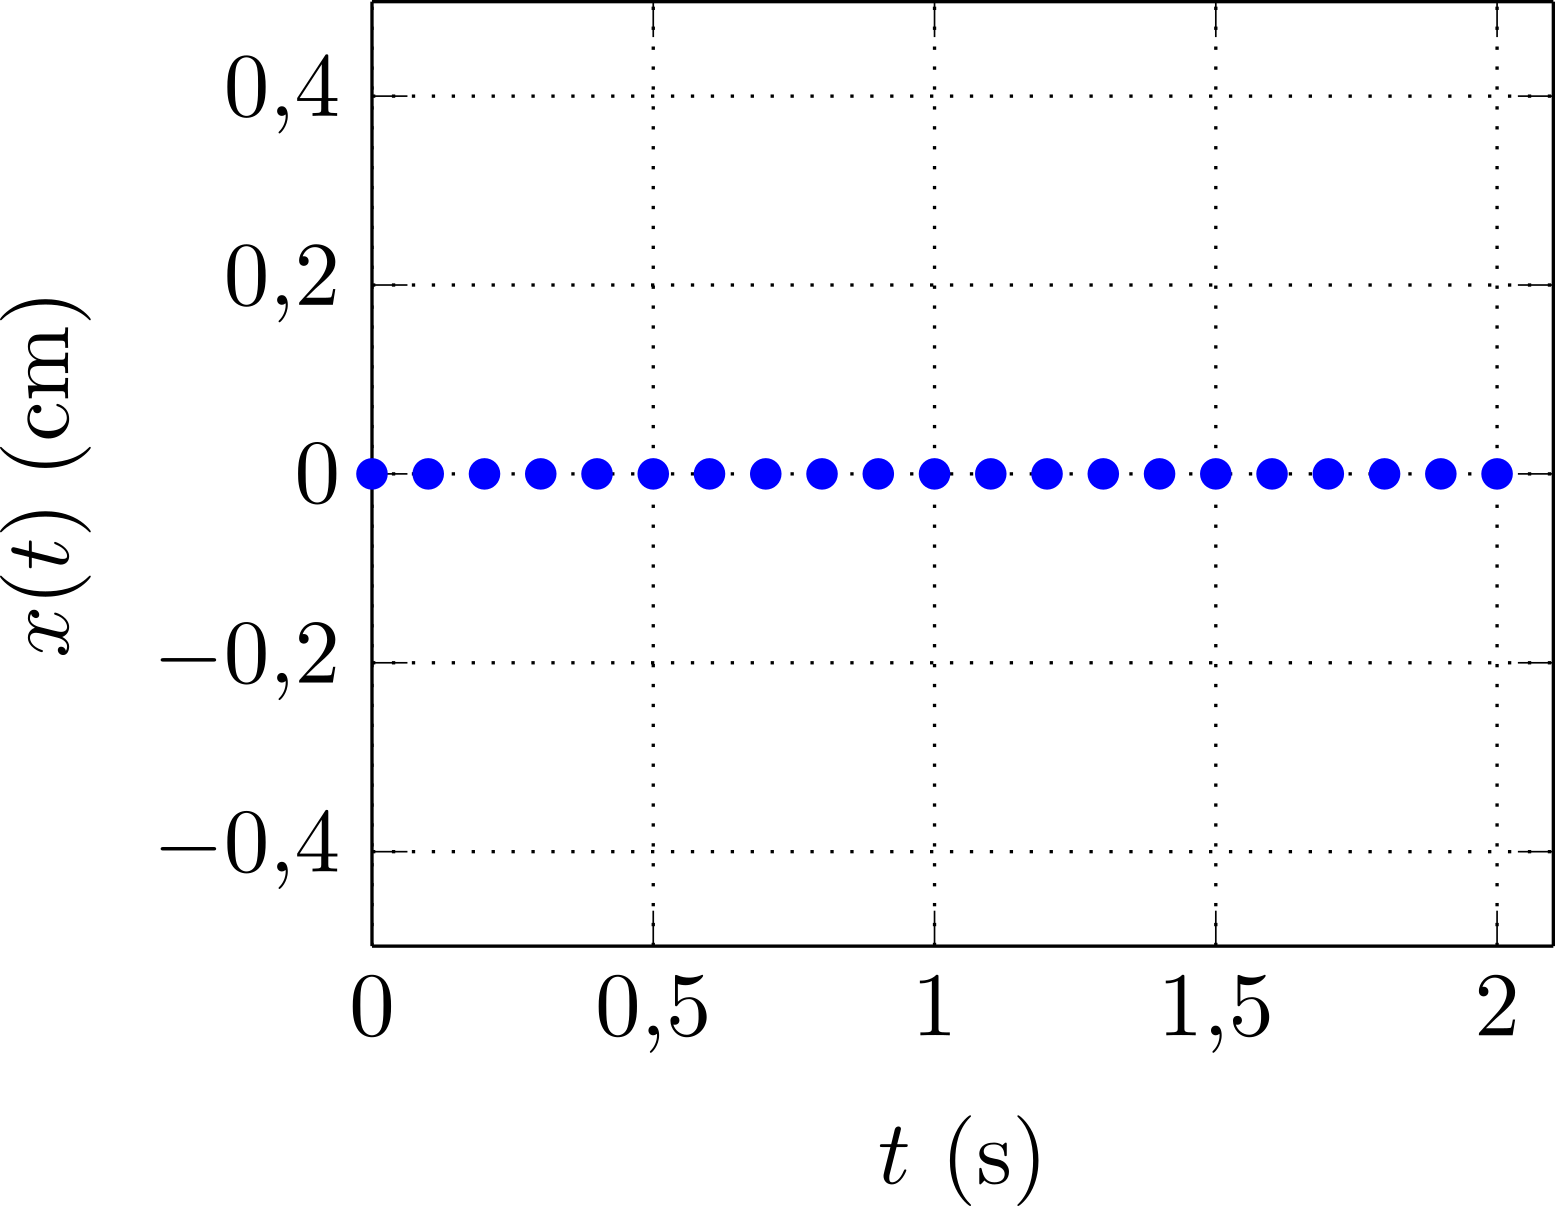
\includegraphics[width=\linewidth]{x_glyc}
		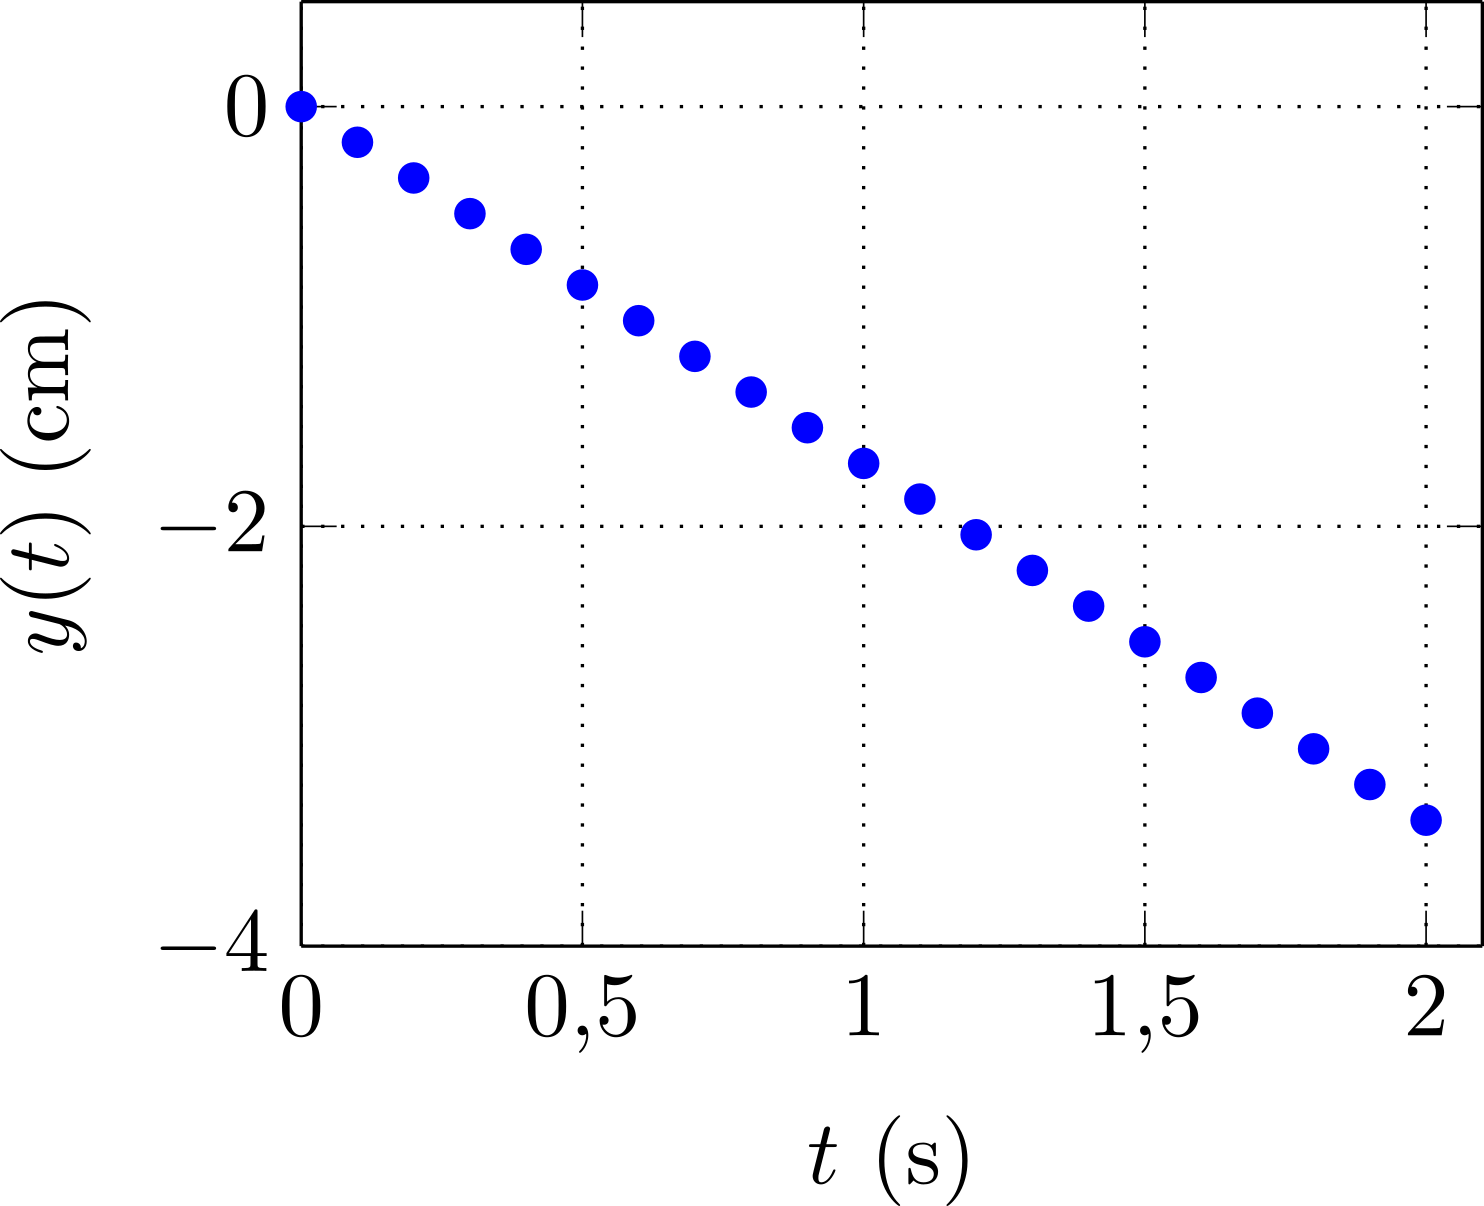
\includegraphics[width=\linewidth]{y_glyc}
	\end{center}
\end{minipage}
\hfill
\begin{minipage}{0.31\linewidth}
	\begin{itemize}
		\item chute libre $v_0 = 0$~:
	\end{itemize}
	\begin{center}
		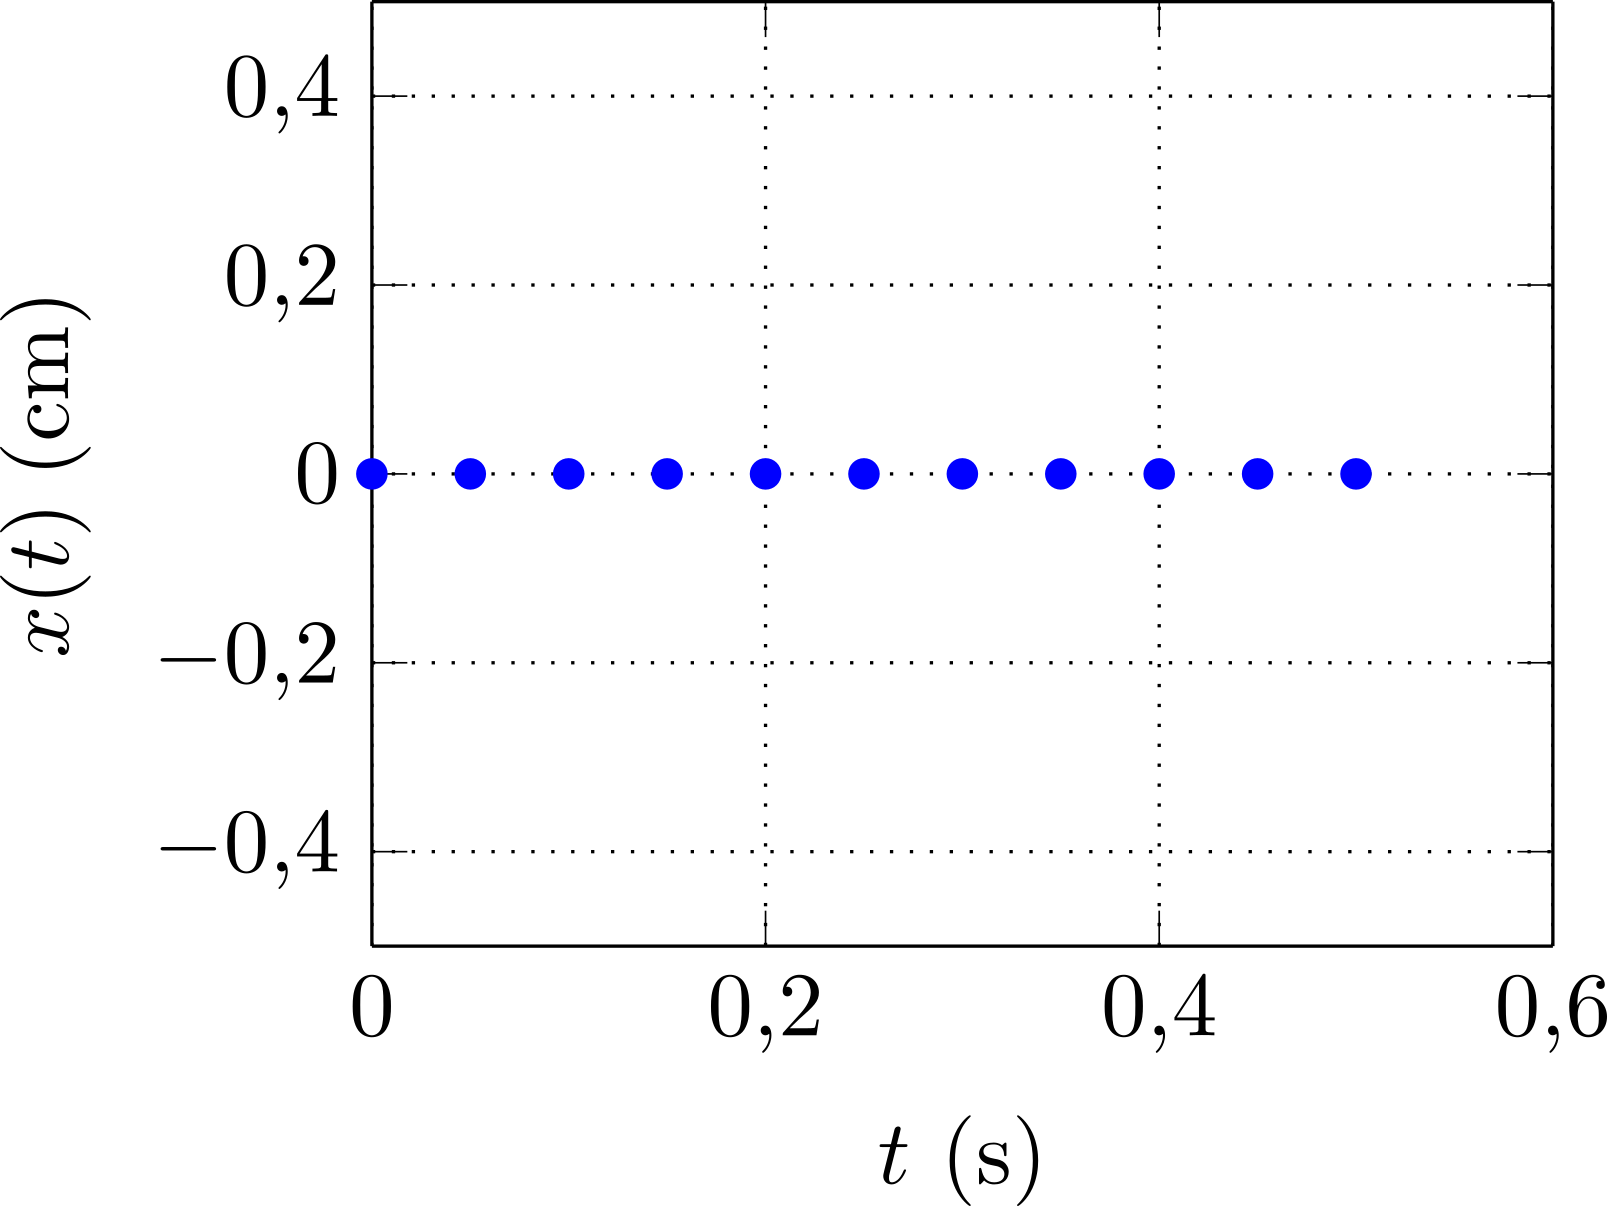
\includegraphics[width=\linewidth]{x_nov}
		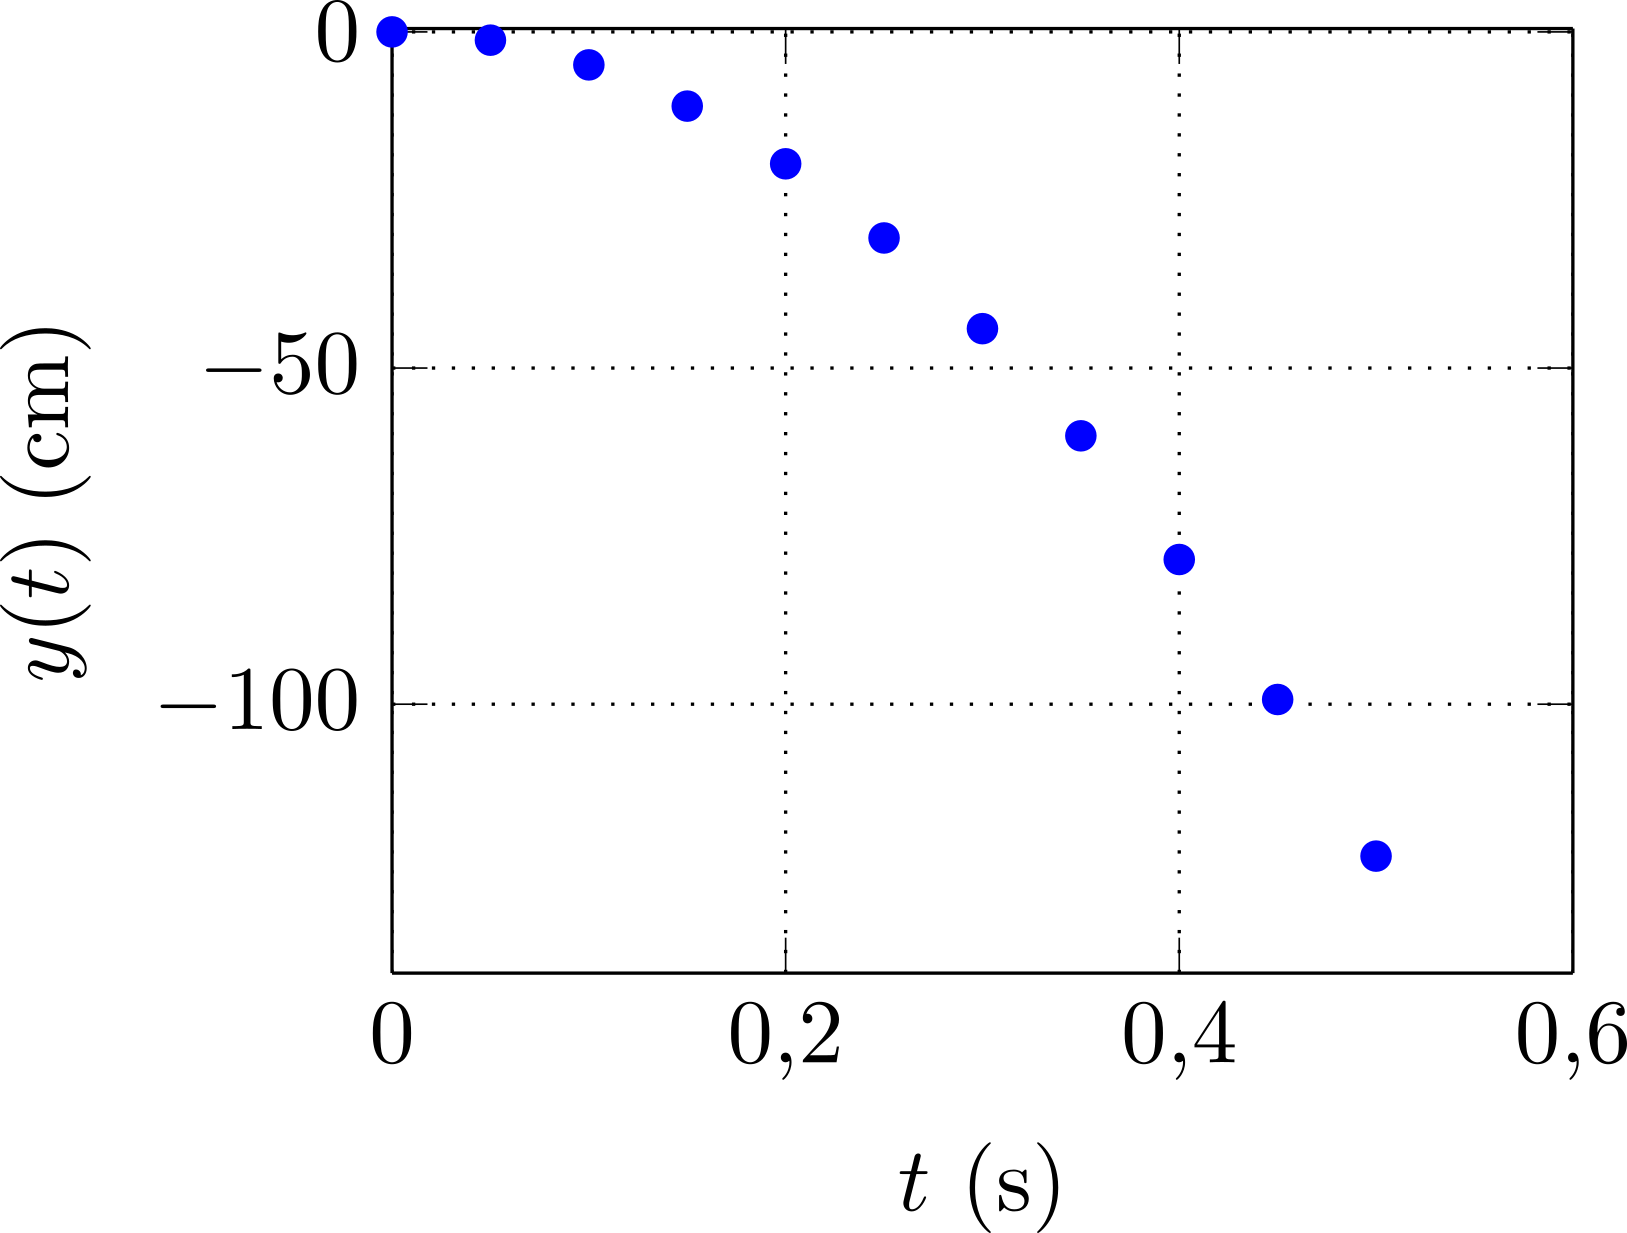
\includegraphics[width=\linewidth]{y_nov}
	\end{center}
\end{minipage}
\hfill
\begin{minipage}{0.31\linewidth}
	\begin{itemize}
		\item chute libre $v_0 \neq 0$~:
	\end{itemize}
	\begin{center}
		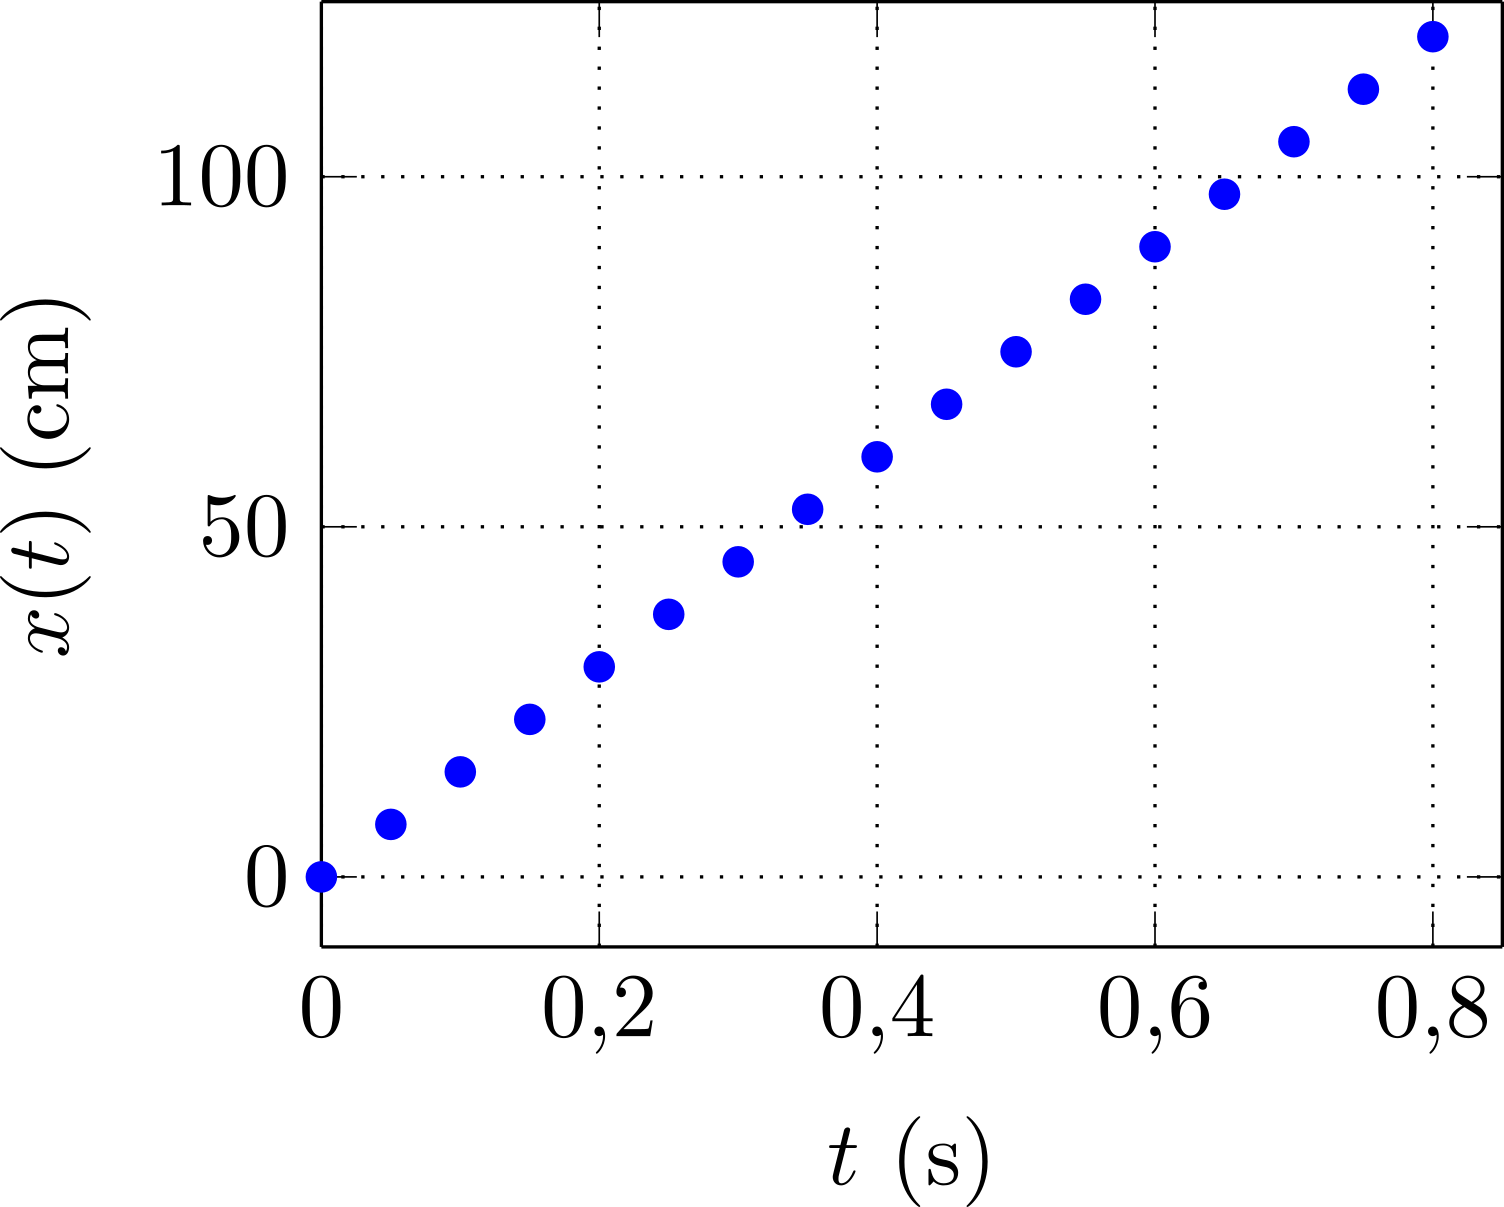
\includegraphics[width=\linewidth]{x_vo}
		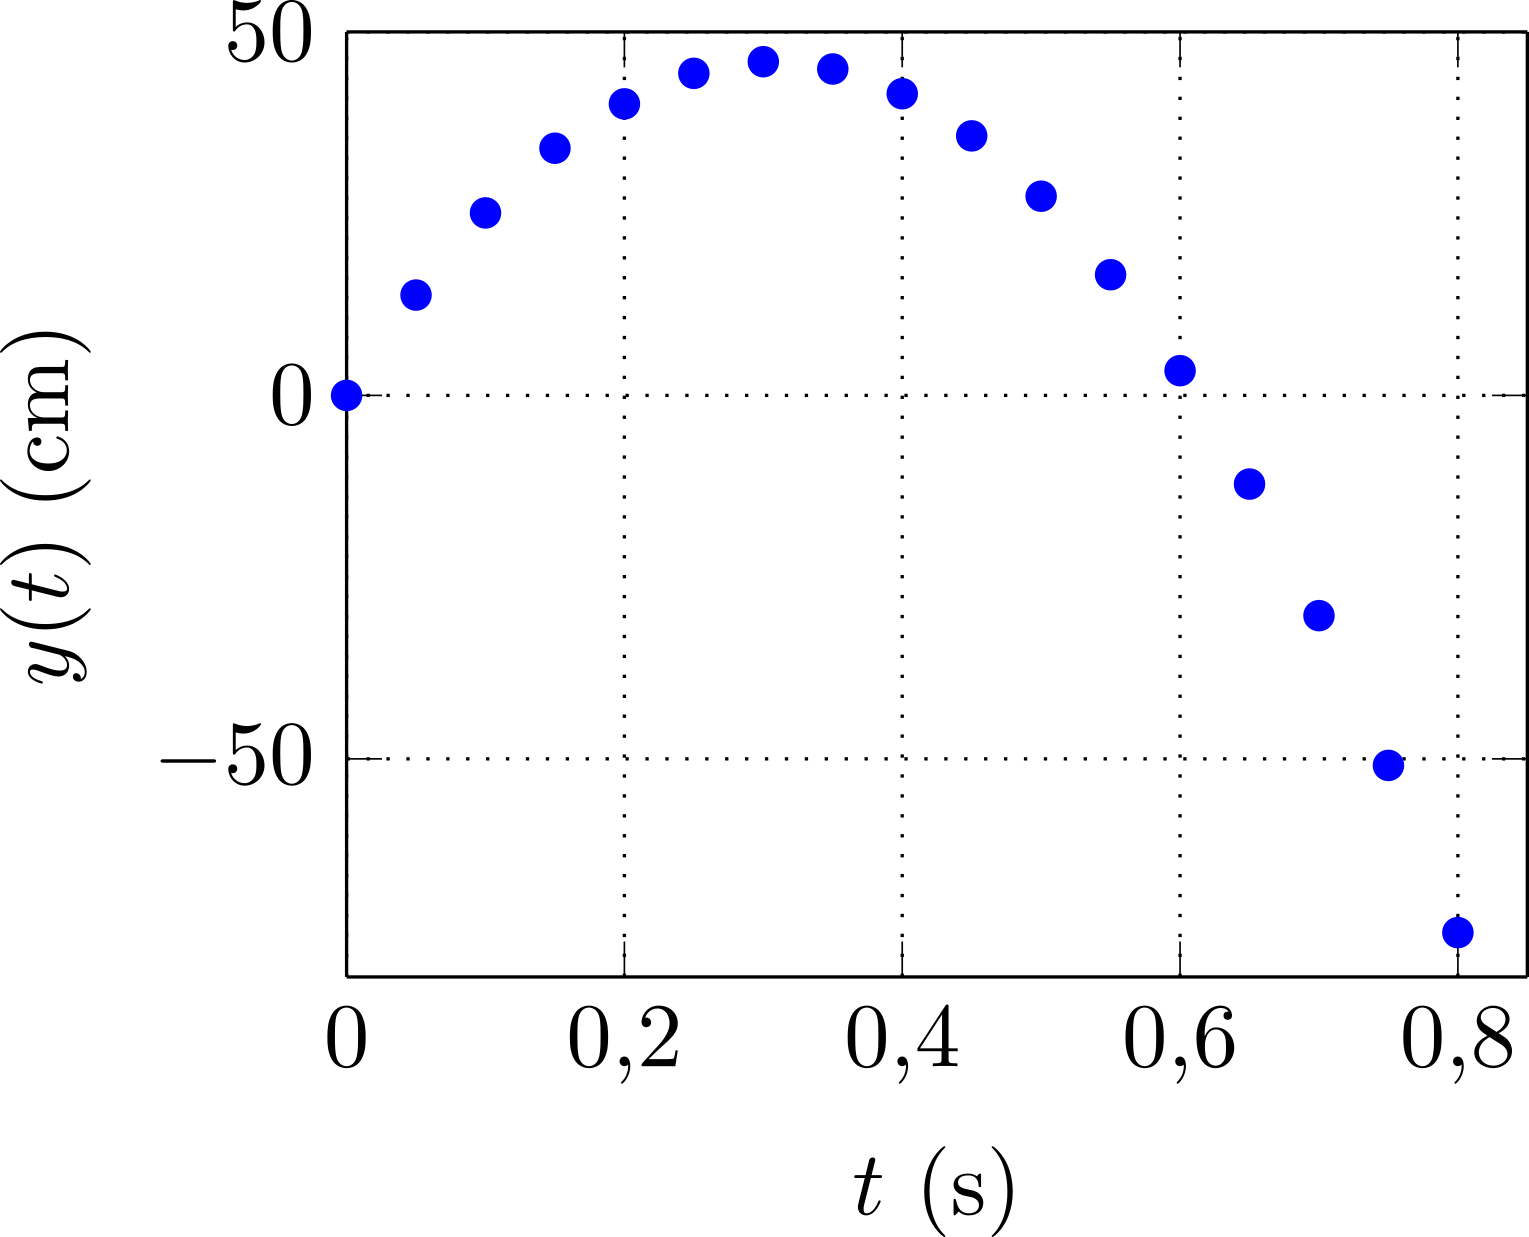
\includegraphics[width=\linewidth]{y_vo}
	\end{center}
\end{minipage}

% \begin{itemize}
%     \item chute dans le glycérol~: \smallbreak
%         \hfill
%         \begin{minipage}{0.35\linewidth}
%             \begin{center}
%                 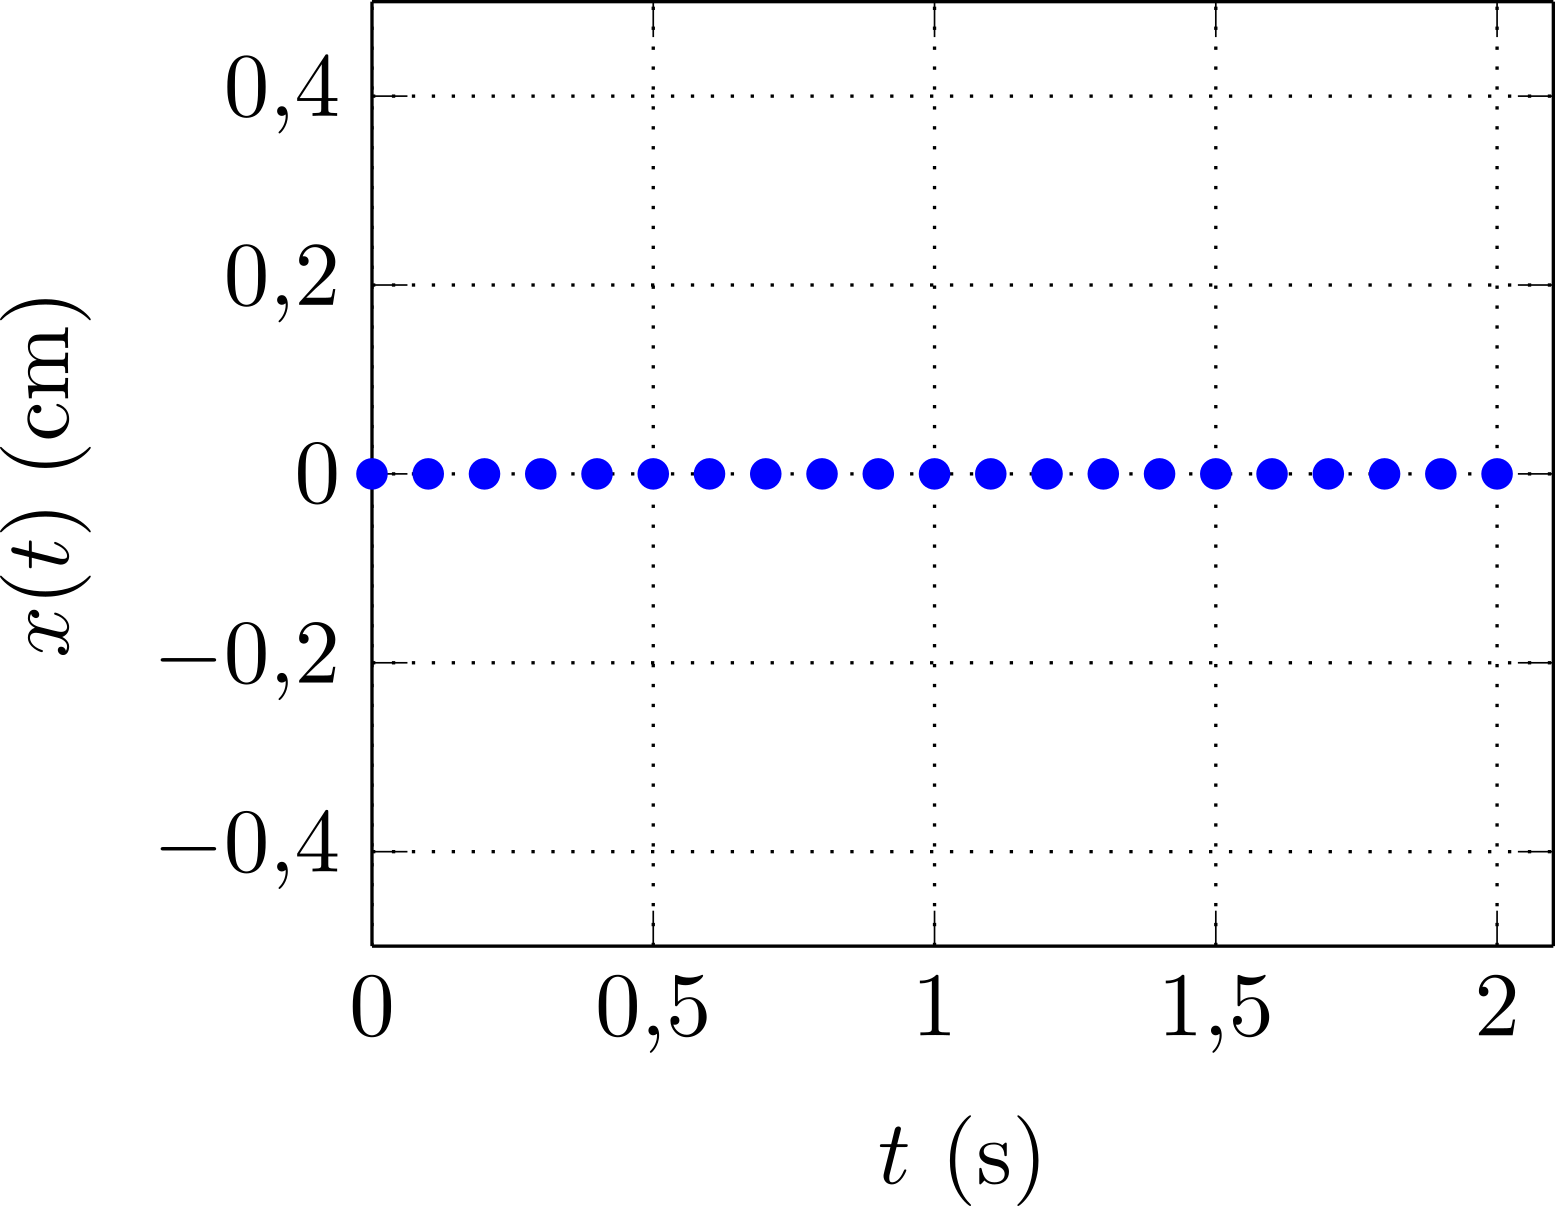
\includegraphics[width=\linewidth]{x_glyc}
%             \end{center}
%         \end{minipage}
%         \begin{minipage}{0.35\linewidth}
%             \begin{center}
%                 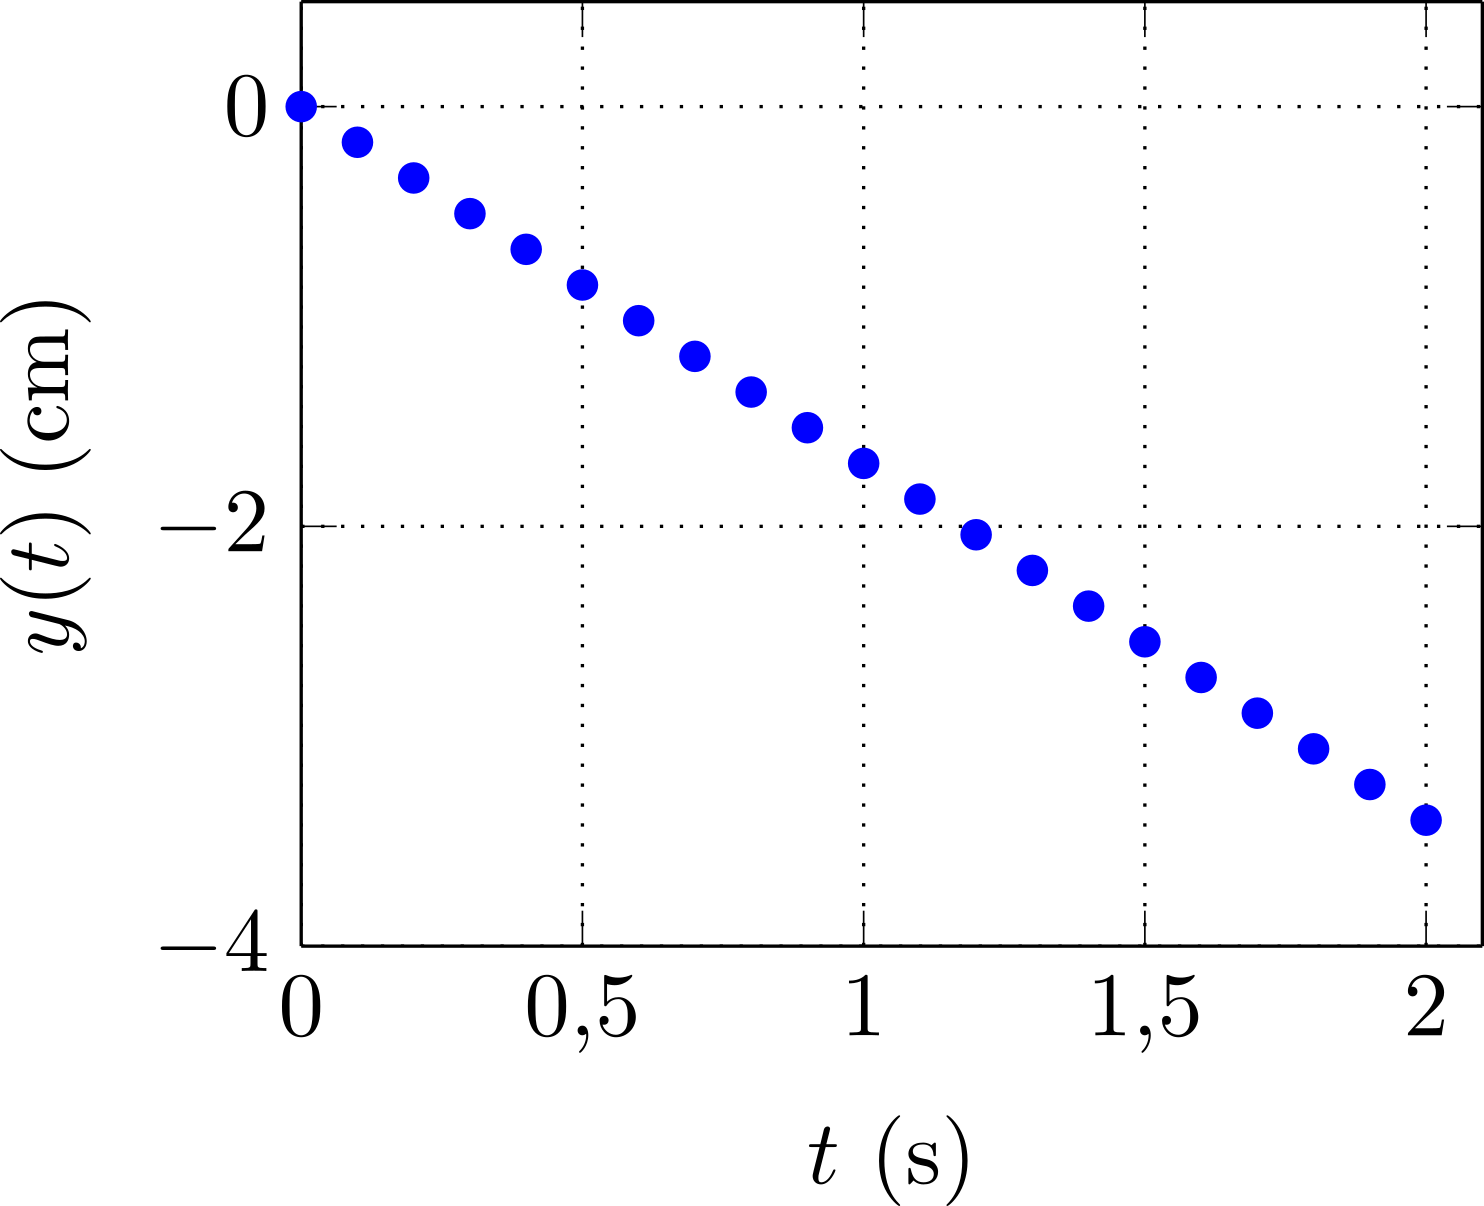
\includegraphics[width=\linewidth]{y_glyc}
%             \end{center}
%         \end{minipage}
%         \hfill~
%     \item chute libre sans vitesse initiale~: \smallbreak
%         \hfill
%         \begin{minipage}{0.35\linewidth}
%             \begin{center}
%                 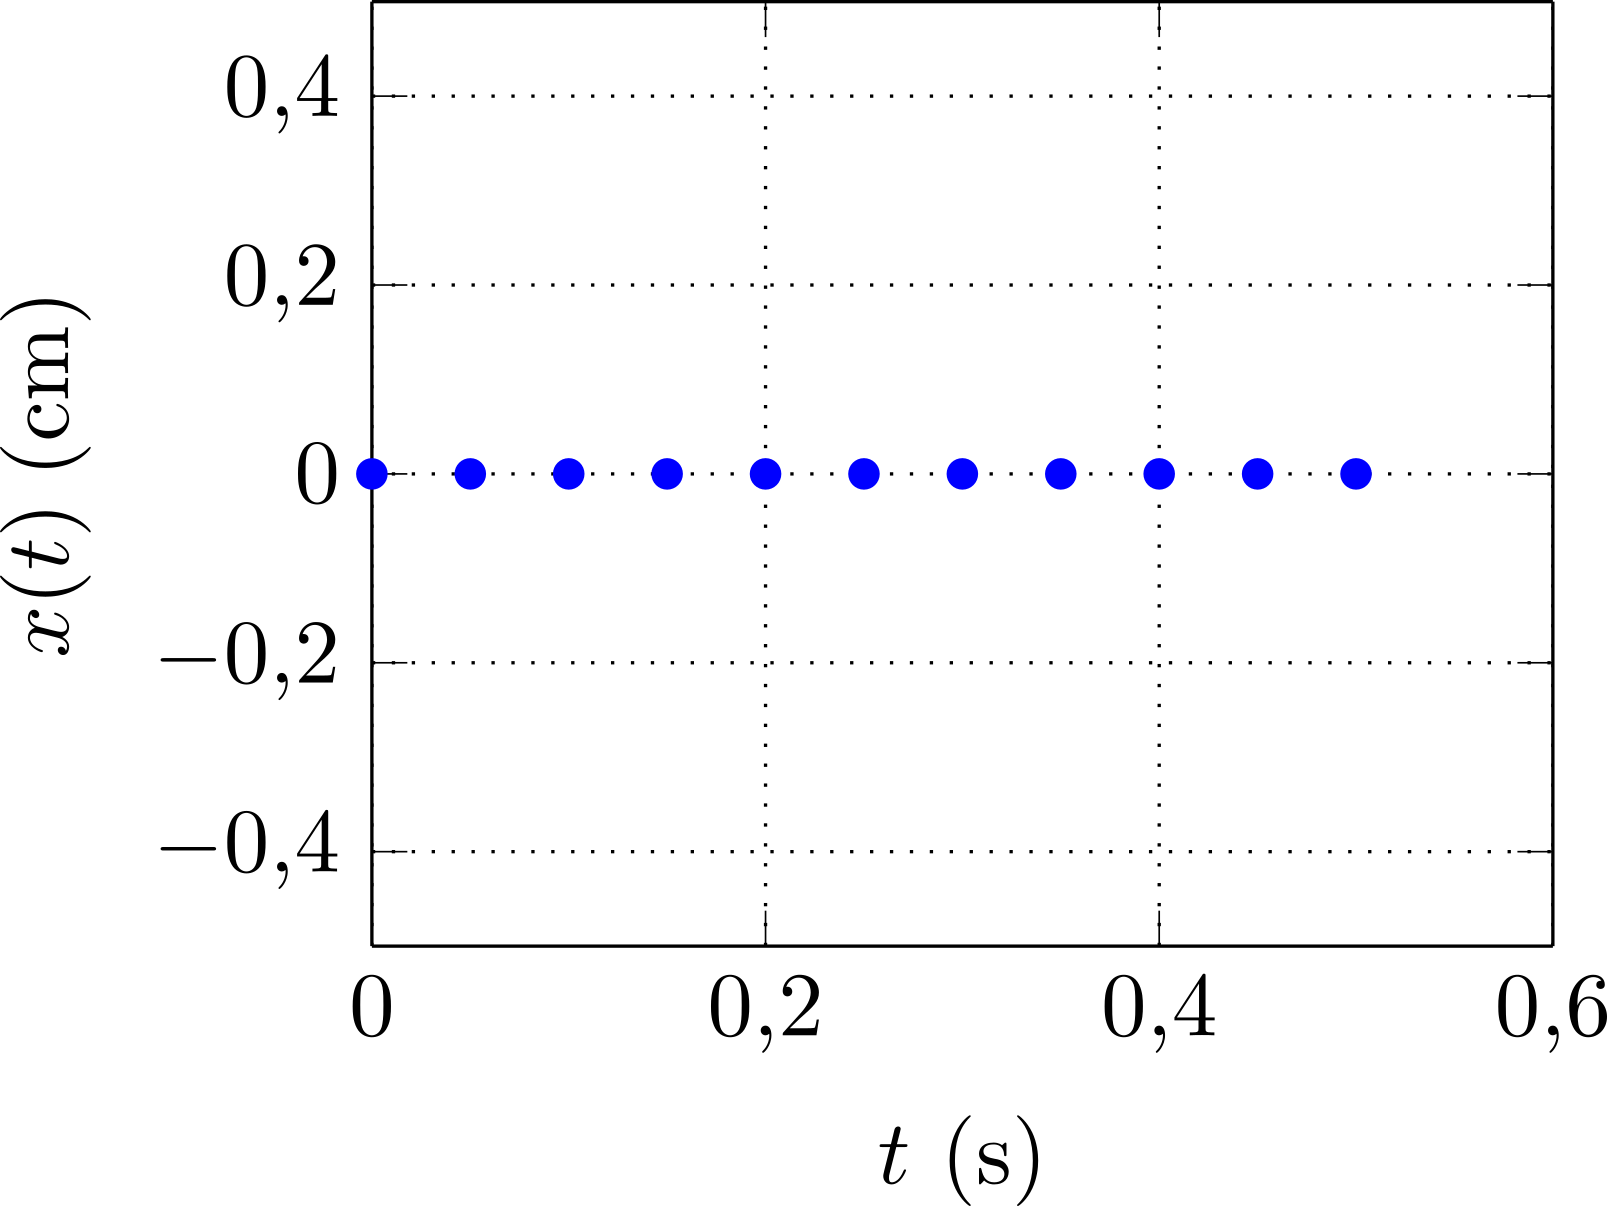
\includegraphics[width=\linewidth]{x_nov}
%             \end{center}
%         \end{minipage}
%         \begin{minipage}{0.35\linewidth}
%             \begin{center}
%                 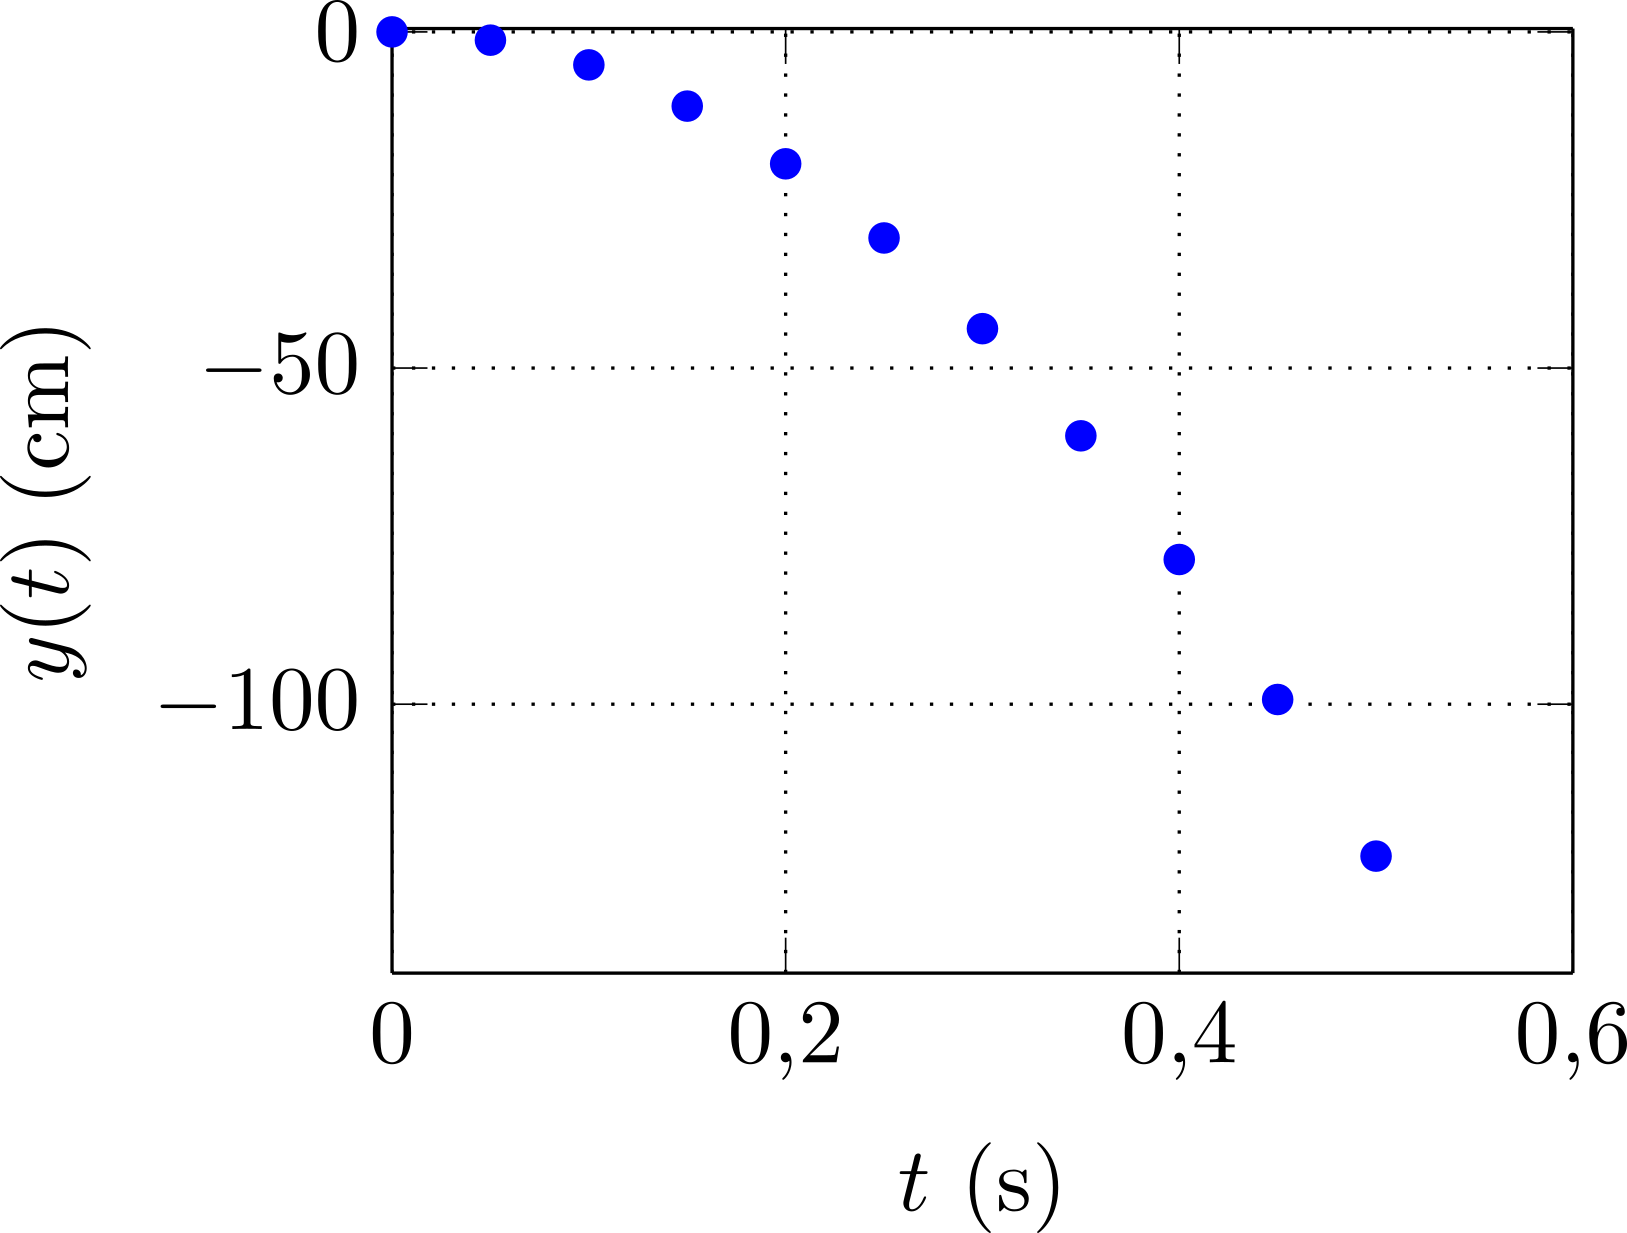
\includegraphics[width=\linewidth]{y_nov}
%             \end{center}
%         \end{minipage}
%         \hfill~
%     \item chute libre avec vitesse initiale~: \smallbreak
%         \hfill
%         \begin{minipage}{0.35\linewidth}
%             \begin{center}
%                 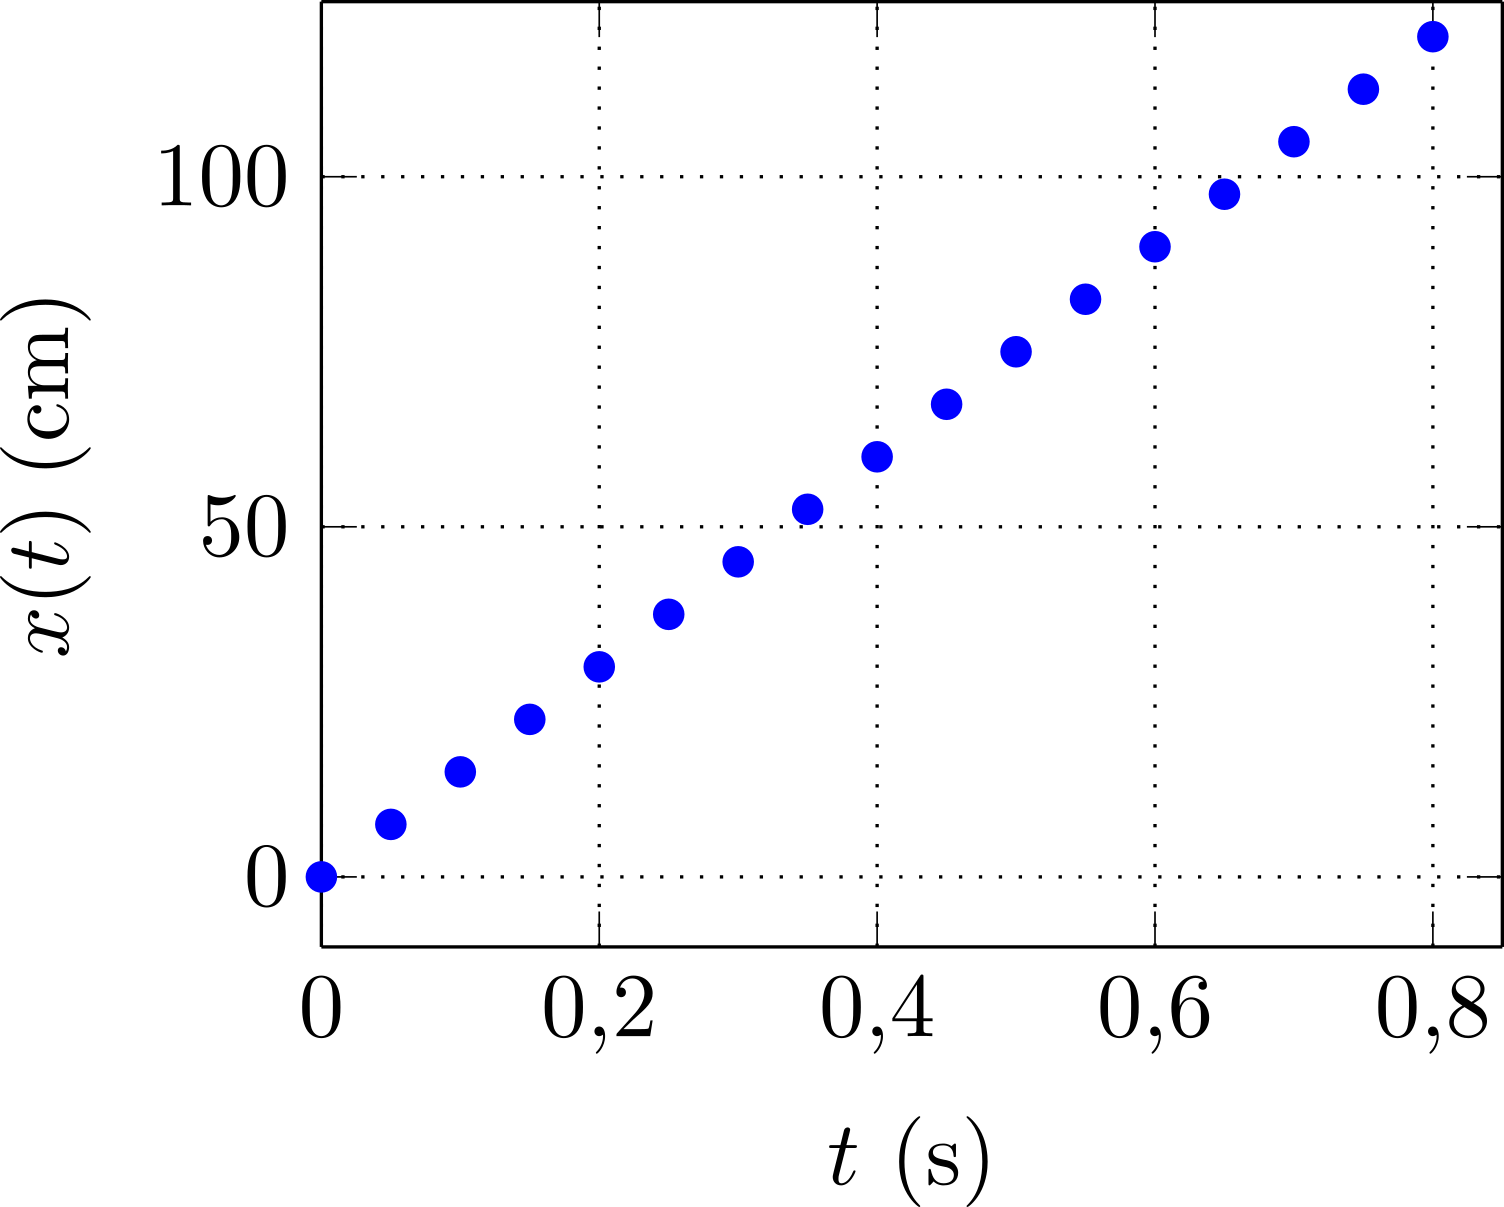
\includegraphics[width=\linewidth]{x_vo}
%             \end{center}
%         \end{minipage}
%         \begin{minipage}{0.35\linewidth}
%             \begin{center}
%                 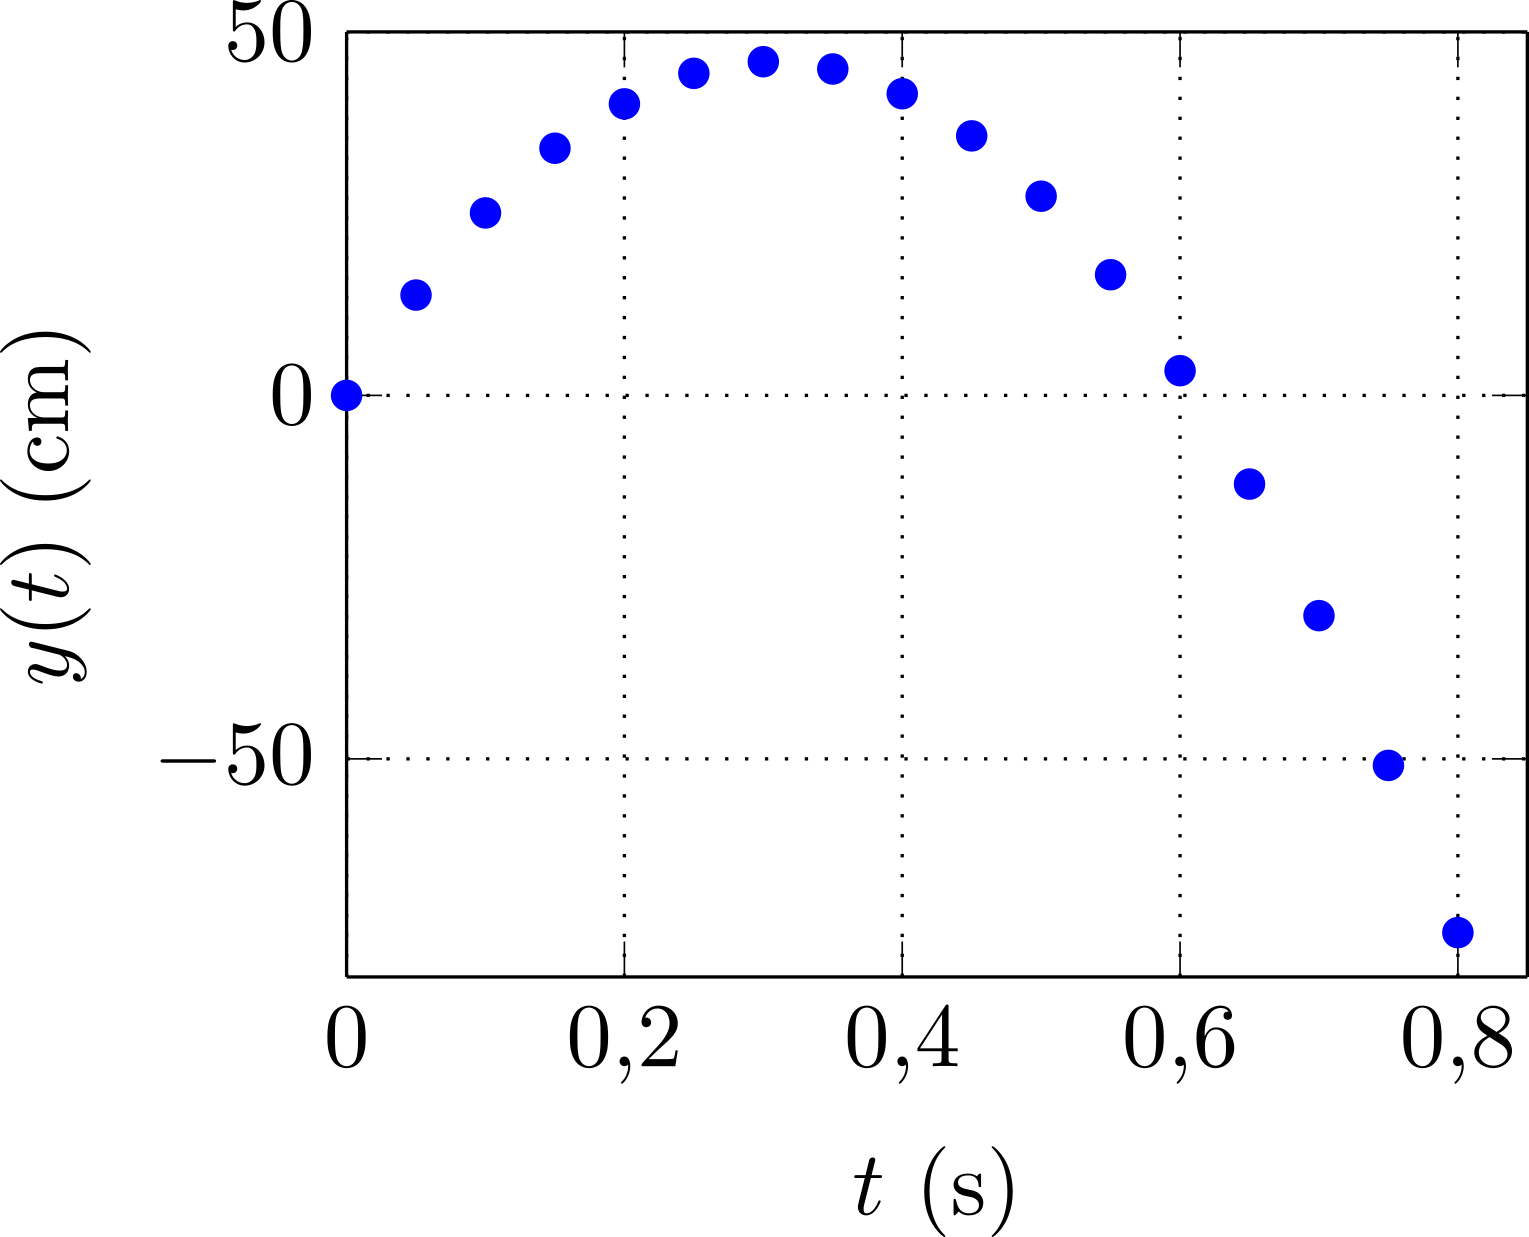
\includegraphics[width=\linewidth]{y_vo}
%             \end{center}
%         \end{minipage}
%         \hfill~
% \end{itemize}

% Les équations horaries peuvent aussi être des expressions analytiques de $x(t)$,
% $y(t)$ et $z(t)$ obtenues à partir d'une modélisation du problème.

\begin{tcb*}(defi)<lfnt>'l'{Trajectoire}
	La \textbf{trajectoire} est l'ensemble des positions successives du point M
	au cours du temps. C'est le «~dessin~» fait par le mobile au cours du temps.
\end{tcb*}

Sur les exemples précédents, la trajectoire est la courbe $y(x)$ car le
mouvement est plan. C'est une droite dans les deux premiers cas, et une parabole
dans le dernier. \bigbreak

\begin{minipage}{0.31\linewidth}
	\begin{center}
		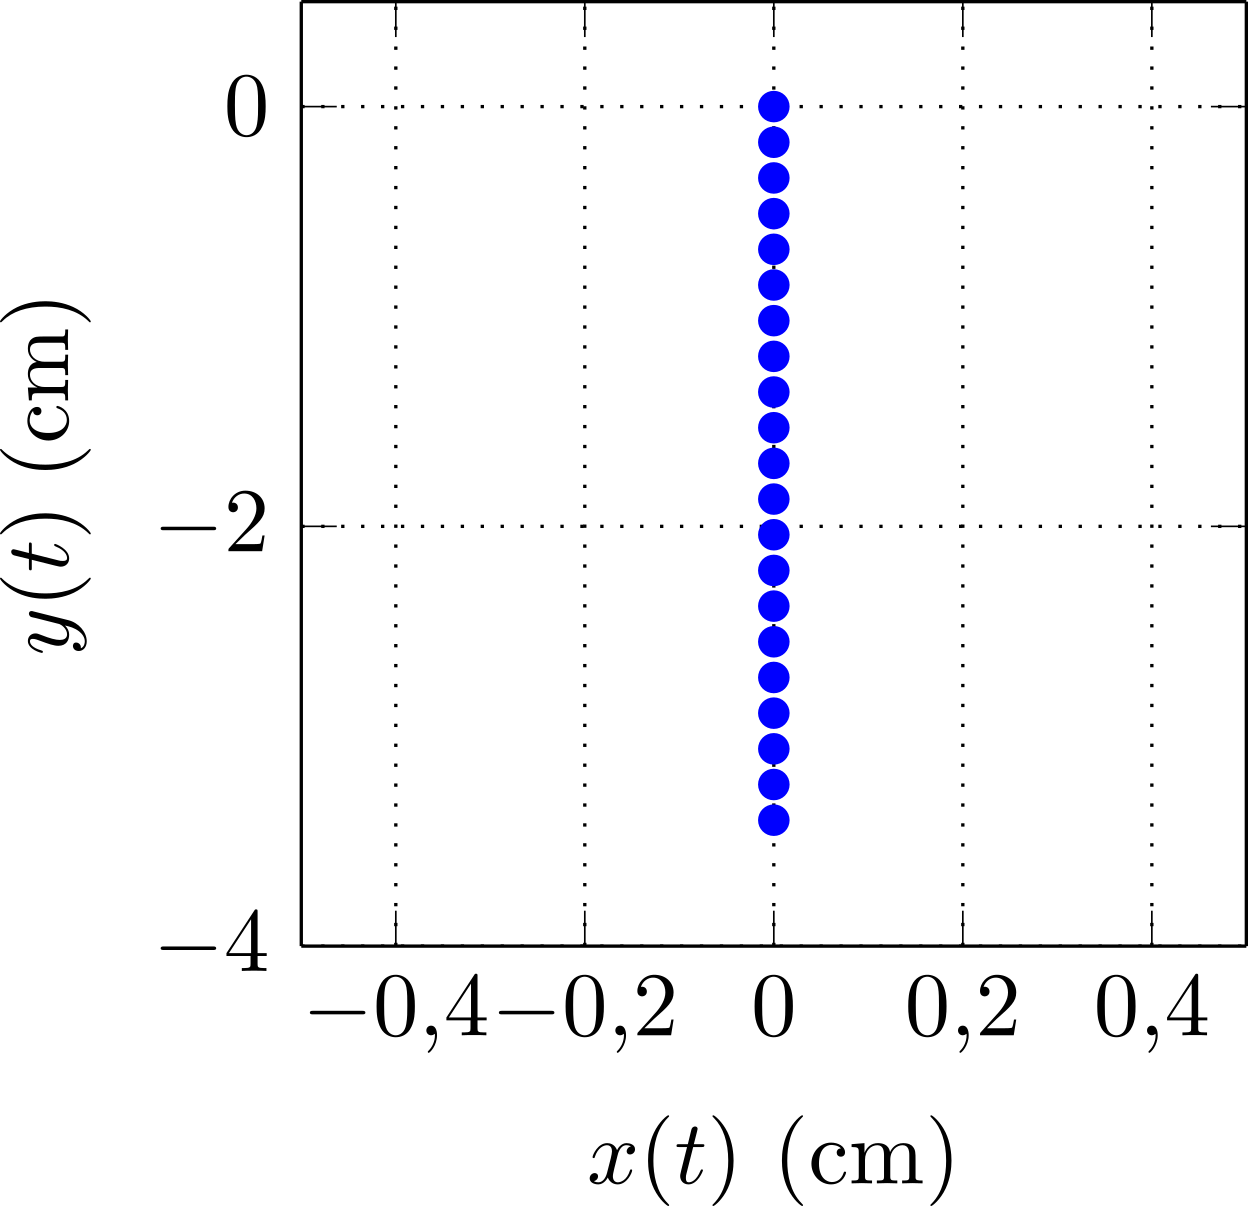
\includegraphics[width=\linewidth]{traj_glyc}
	\end{center}
\end{minipage}
\hfill
\begin{minipage}{0.31\linewidth}
	\begin{center}
		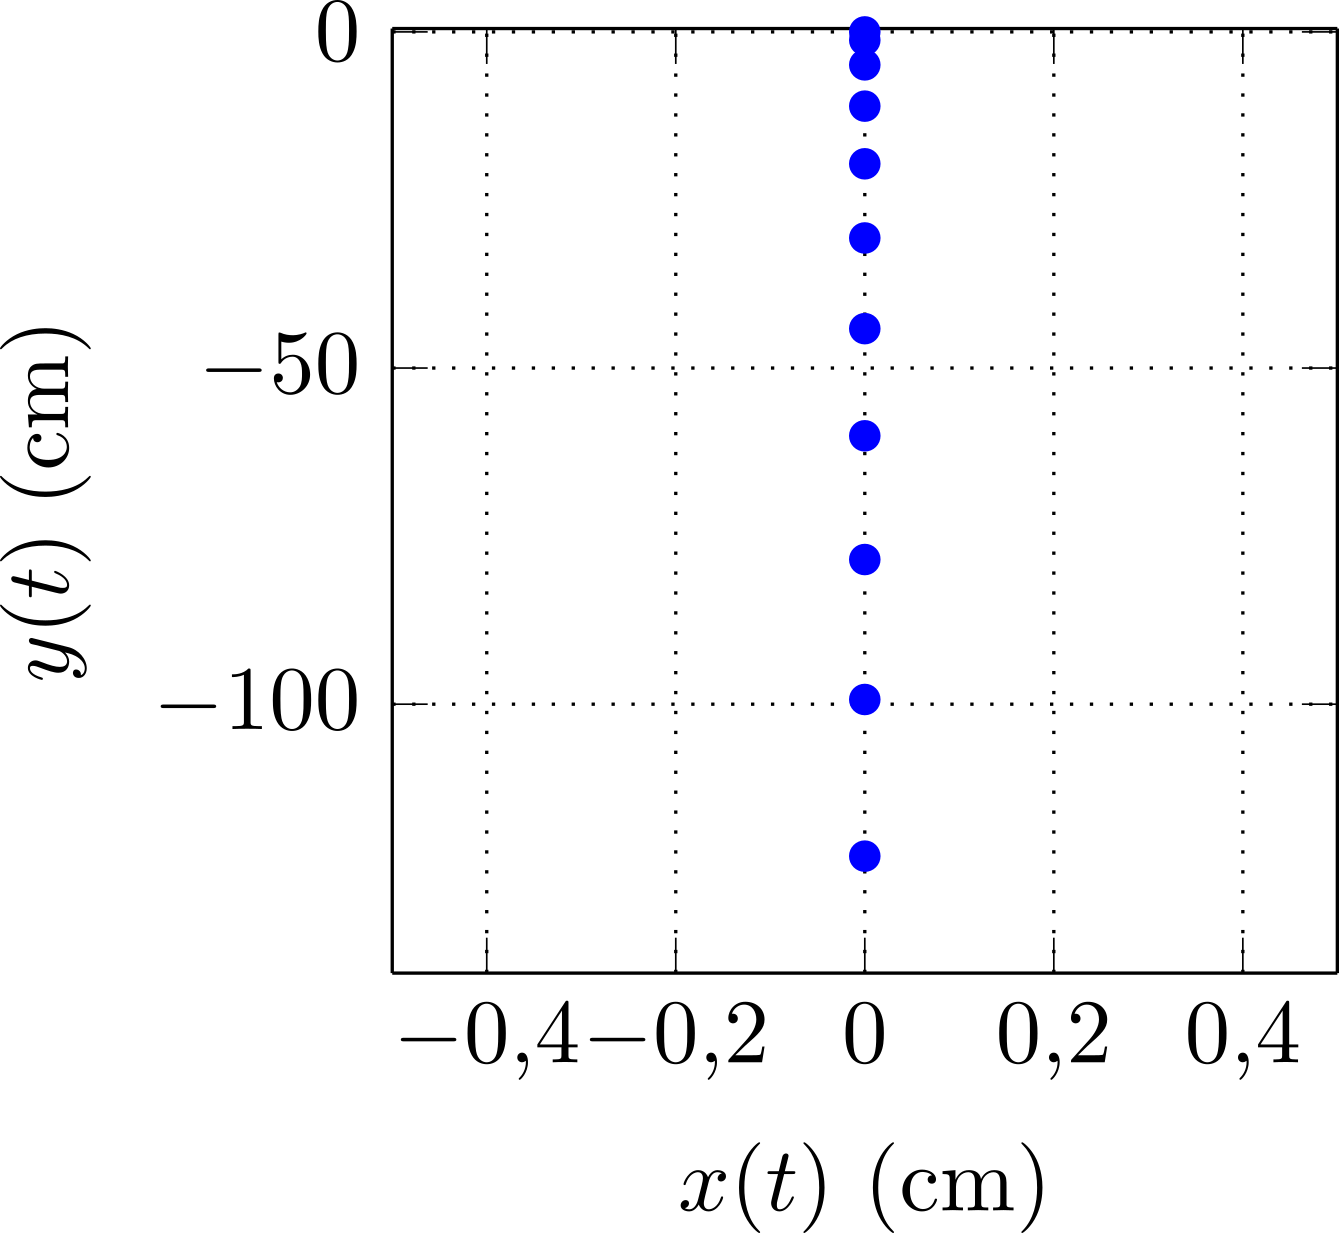
\includegraphics[width=\linewidth]{traj_nov}
	\end{center}
\end{minipage}
\hfill
\begin{minipage}{0.31\linewidth}
	\begin{center}
		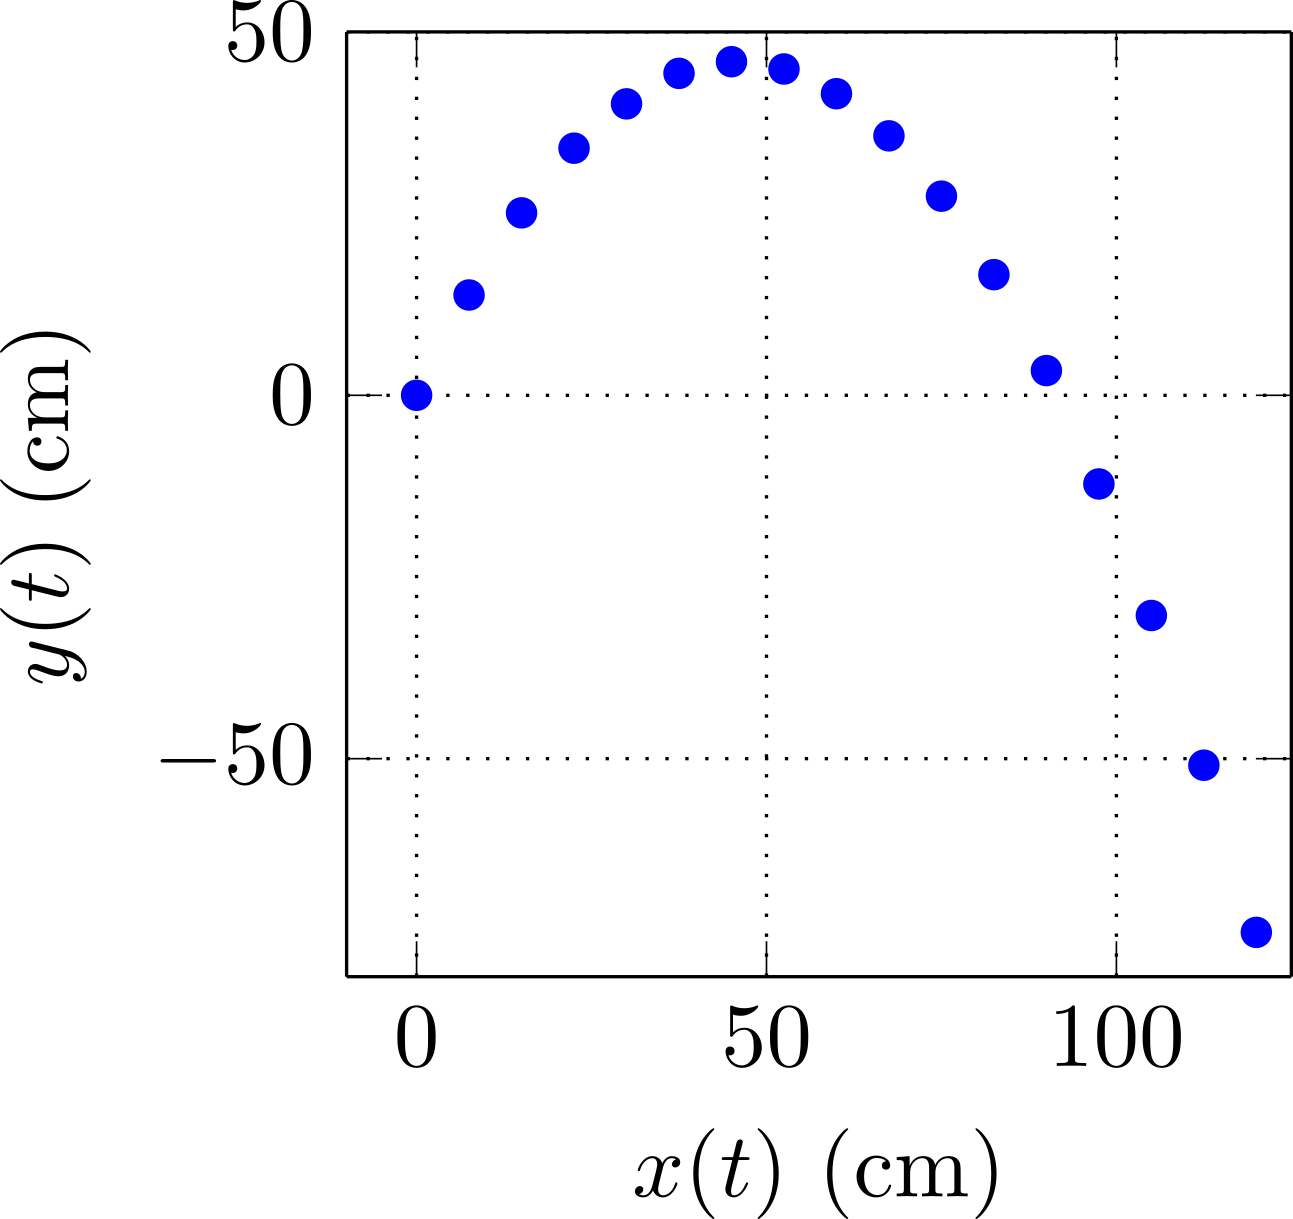
\includegraphics[width=\linewidth]{traj_vo}
	\end{center}
\end{minipage}

\subsection{Vitesse}
\begin{tcb*}[sidebyside, righthand ratio=.29](defi){Vitesses}
	On définit la \textbf{vitesse} comme le \textbf{taux d'accroissement} du
	vecteur position~:
	\[\psw{\boxed{\vf(t) = \frac{\OM(t+\Dt) - \OM(t)}{\Dt}}}
		\qdonc
		[\vf] = \si{m.s^{-1}}\]
	Si on effectue des mesures très rapprochées, c'est-à-dire $\Dt \rightarrow
		0$, on définit alors la vitesse \textit{instantanée} par~:
	\[\psw{\boxed{\vf(t) = \dv{\OM(t)}{t}}}\]
	\tcblower
	\begin{center}
		\sswitch{
			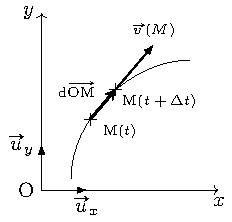
\includegraphics[width=\linewidth, draft=true]{vec_vit}
		}{
			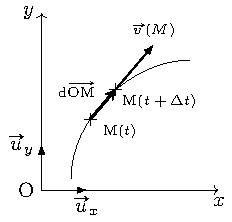
\includegraphics[width=\linewidth]{vec_vit}
		}
		\captionof{figure}{Vecteur vitesse.}
	\end{center}
\end{tcb*}

\begin{tcb*}[cnt, bld](ror){Vitesse et trajectoire}
	Le vecteur vitesse est toujours tangent à la trajectoire.
\end{tcb*}

On peut donc voir la vitesse comme étant le rapport du déplacement élémentaire
par la durée infinitésimal $\dd{t}$, ou comme étant la dérivée du vecteur
position.
\smallbreak
Ainsi, si le vecteur position est
\[
	\OM(t) = x(t)\ux + y(t)\uy + z(t)\uz
	\Ra
	\dd{\OM} = \dd{x}\ux + \dd{y}\uy + \dd{z}\uz
\]
alors dans la vision dérivative, on obtient
\[\vf(t) = \dv{t}\left(x(t)\ux + y(t)\uy + z(t)\uz\right)\]
Or, \textbf{en coordonnées cartésiennes}, les vecteurs de base ne varient pas
avec le temps~: il ne changent pas de direction et restent unitaires. On peut
donc les considérer comme des constantes multiplicatives, et ainsi
\[\psw{\vf(t) = \dv{x}{t}(t)\ux + \dv{y}{t}(t)\uy + \dv{z}{t}(t)\uz}\]
On obtient la même chose avec la vision rapport déplacement/temps.
Pour alléger l'écriture, on introduit une notation~:
\begin{tcb*}(nota)<lfnt>'l'{Dérivée temporelle en mécanique}
	En mécanique, les dérivées \textbf{par rapport au temps} se notent avec un
	point sur la fonction~:
	\[\dv{x}{t}(t) = \xp(t)\]
\end{tcb*}
Ainsi, on trouve
\[\psw{\boxed{\vf(t) = \xp(t)\ux + \yp(t)\uy + \zp(t)\uz}}\]

\begin{tcb*}(exem)<lfnt>'l'{Vitesse selon expérience}
	En reprenant les exemples précédents~:
	\begin{itemize}
		\item Pour la chute dans le glycérol, $\xp = 0$ et $\yp = \cte$. Ainsi,
		      $\vf$ est constant, et dirigé vers le bas.
		\item Pour la chute libre sans vitesse initiale, $\xp = 0$ et $\yp$
		      diminue linéairement~: le vecteur vitesse est variable, dirigé vers
		      le bas.
		\item Pour la chute libre avec vitesse initiale, $\xp = \cte$ et $\yp$
		      diminue linéairement~: le vecteur vitesse est variable et change de
		      direction.
	\end{itemize}
\end{tcb*}

\begin{tcb*}(impo){Différence vecteur/norme}
	Selon le contexte, on fera particulièrement attention à ne pas confondre le
	mot «~vitesse~» avec le \textbf{vecteur} ou avec sa \textbf{norme}. Une
	vitesse, en norme, ne saurait être négative~; un vecteur vitesse peut être
	négatif.
\end{tcb*}

\subsection{Accélération}
L'accélération est la grandeur physique qui mesure la variation de la vitesse.
\begin{tcb*}(defi){Accélérations}
	On définit l'\textbf{accélération} comme le \textbf{taux d'accroissement} du
	vecteur vitesse~:
	\[\psw{\boxed{\af(t) = \frac{\vf(t+\Dt) - \vf(t)}{\Dt}}}
		\qdonc
		[\af] = \si{m.s^{-2}}\]
	Si on effectue des mesures très rapprochées, c'est-à-dire $\Dt \rightarrow
		0$, on définit alors l'accélération \textit{instantanée} comme étant la
	\textit{dérivée} du vecteur vitesse, et dérivée seconde de la position~:
	\[\psw{\boxed{\af(t) = \dv{\vf(t)}{t}}}
		\qet
		\psw{\boxed{\af(t) = \dv[2]{\OM(t)}{t}}}\]
\end{tcb*}

\begin{tcb*}[cnt, bld](ror){Accélération et trajectoire}
	Le vecteur accélérations est toujours dirigé vers l'intérieur à la
	trajectoire (partie concave).
\end{tcb*}

Par distribution de l'opérateur $\dv{t}$, on obtient en cartésiennes
\[\psw{\boxed{\af(t) = \xpp(t)\ux + \ypp(t)\uy + \zpp(t)\uz}}\]

\begin{tcb*}(exem)<lfnt>'l'{Accélération selon expérience}
	En reprenant les exemples précédents~:
	\begin{itemize}
		\item Pour la chute dans le glycérol, $\xpp$ et $\ypp$ sont nuls~: le
		      vecteur accélération est nul.
		\item Pour la chute libre sans vitesse initiale, $\xpp = 0$ et $\ypp$
		      est constant~: le vecteur accélération est constant, dirigé vers le
		      bas.
		\item Pour la chute libre avec vitesse initiale, $\xpp = 0$ et $\ypp$
		      est constant~: le vecteur accélération est constant, dirigé vers le
		      bas.
	\end{itemize}
\end{tcb*}

\begin{tcb*}(impo){Accélération}
	Une accélération peut être négative ou nulle~:
	\begin{itemize}
		\item En physique l'accélération est liée à la \textbf{variation du
			      vecteur vitesse}, souvent différent de l'utilisation courante de ce
		      mot.
		\item Pour que l'accélération soit nulle, il faut que toutes les
		      composantes de la vitesse ne varient pas. Un mouvement peut être à
		      vitesse constante en norme, mais d'accélération non nulle.
	\end{itemize}
\end{tcb*}

\section{Exemples de mouvements}
% \subsection{Rappel mathématique}
% \begin{tcb}(rapp)<lft>'l'{Rappel}
% 	\begin{itemize}
% 		\item Si $\xp(t) = 0$, alors $x(t) = x_0$ avec $x_0 = \cte$.
% 		\item Si $\xp(t) = v_0$, alors $x(t) = v_0t + x_0$ avec $x_0 = \cte$.
% 		\item Si $\xp(t) = a_0t$, alors $x(t) = \DS \frac{1}{2}a_0t^2 +  x_0$
% 		      avec $x_0 = \cte$.
% 	\end{itemize}
% \end{tcb}

\subsection{Mouvement rectiligne uniforme}
\begin{tcb*}(defi)<lfnt>'l'{Mouvement rectiligne uniforme}
	Un mouvement est dit \textbf{uniforme} si la \textbf{norme du vecteur vitesse}
	$\norm{\vf}$ est constante. Il est dit \xul{rectiligne} si la \xul{trajectoire
		est une droite}.
\end{tcb*}
Par exemple,
\[\vf = v_0\ux\]
donne un mouvement rectiligne uniforme. C'est le cas de la chute dans le
glycérol. Dans ce cas,
\psw{
	\[
		\left\{
		\begin{array}{l}
			\xp(t) = v_0 \\
			\yp(t) = 0   \\
			\zp(t) = 0
		\end{array}
		\right.
		\Longrightarrow
		\left\{
		\begin{array}{l}
			x(t) = v_0t + x_0 \\
			y(t) = y_0        \\
			z(t) = z_0
		\end{array}
		\right.
	\]}
avec $x_0$, $y_0$ et $z_0$ des constantes que l'on peut calculer à l'aide des
conditions initiales.

\subsection{Mouvement rectiligne uniformément accéléré}
\begin{tcb*}(defi)<lfnt>'l'{Uniformément accéléré}
	Un mouvement est dit \textit{uniformément accéléré} si la \textbf{norme du
		vecteur accélération} $\norm{\af}$ est constant.
\end{tcb*}
Par exemple,
\[\af = -g\uy\]
avec des conditions initiales nulles donne un mouvement rectiligne uniformément
accéléré. C'est le cas de la chute libre sans vitesse initiale. Contextualisons
l'étude~:
\smallbreak
\noindent
\begin{minipage}{0.80\linewidth}
	\begin{itemize}
		\bitem{Système}~: \psw{point matériel.}
		\bitem{Référentiel}~: \psw{celui du laboratoire, supposé galiléen.}
		\bitem{Repère}~: \psw{cartésien avec $\uy$ verticale
			ascendante.}
		\bitem{Origine des temps}~:
		\psw{le moment où la balle est lâchée, tel que $\vf(0) = \of$.}
		\bitem{Origine du repère}~:
		\psw{O tel que $\OM(0) = \of$.}
	\end{itemize}
\end{minipage}
\hfill
\begin{minipage}{0.19\linewidth}
	\begin{center}
		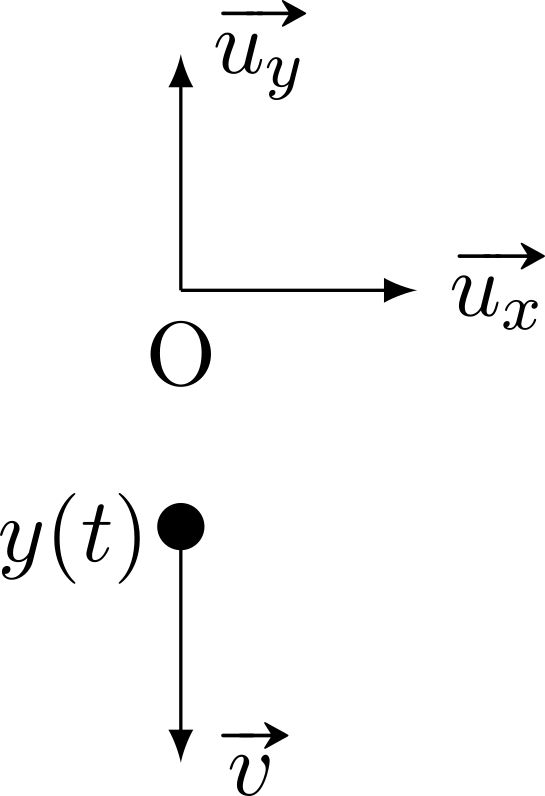
\includegraphics[height=3cm]{nov_init}
		\captionof{figure}{Situation initiale.}
	\end{center}
\end{minipage}

Par définition,
\[\psw{\af(t) = \xpp(t)\ux + \ypp(t)\uy + \zpp(t)\uz}\]
Soit
\[
	\psw{
		\left\{
		\begin{array}{l}
			\xpp(t) = 0  \\
			\ypp(t) = -g \\
			\zpp(t) = 0
		\end{array}
		\right.
		\Longrightarrow
		\left\{
		\begin{array}{l}
			\xp(t) = v_{x,0}       \\
			\yp(t) = -gt + v_{y,0} \\
			\zp(t) = v_{z,0}
		\end{array}
		\right.
	}\]
Or,
\[\psw{
		\vf(0) = \of
		\qdonc
		\left\{
		\begin{array}{l}
			\xp(0) = v_{x,0} = 0 \\
			\yp(0) = v_{y,0} = 0 \\
			\zp(0) = v_{z,0} = 0
		\end{array}
		\right.
	}\]
Ainsi
\[
	\psw{
		\left\{
		\begin{array}{l}
			\xp(t) = 0   \\
			\yp(t) = -gt \\
			\zp(t) = 0
		\end{array}
		\right.
		\Longrightarrow
		\left\{
		\begin{array}{l}
			x(t) = x_{0}                     \\
			y(t) = -\dfrac{1}{2}gt^2 + y_{0} \\
			z(t) = z_{0}
		\end{array}
		\right.
	}\]
Seulement,
\[\psw{
		\OM(0) = \of
		\qdonc
		\left\{
		\begin{array}{l}
			x(0) = y_{0} = 0 \\
			y(0) = y_{0} = 0 \\
			z(0) = z_{0} = 0
		\end{array}
		\right.
	}\]
Autrement dit,
\[\psw{
		\boxed{
			\left\{
			\begin{array}{l}
				x(t) = 0                 \\
				y(t) = -\dfrac{1}{2}gt^2 \\
				z(t) = 0
			\end{array}
			\right.
		}}\]
Ce sont les équations horaires du mouvement, décrivant une droite dans l'espace.

\hfill
\begin{minipage}{0.45\linewidth}
	\begin{center}
		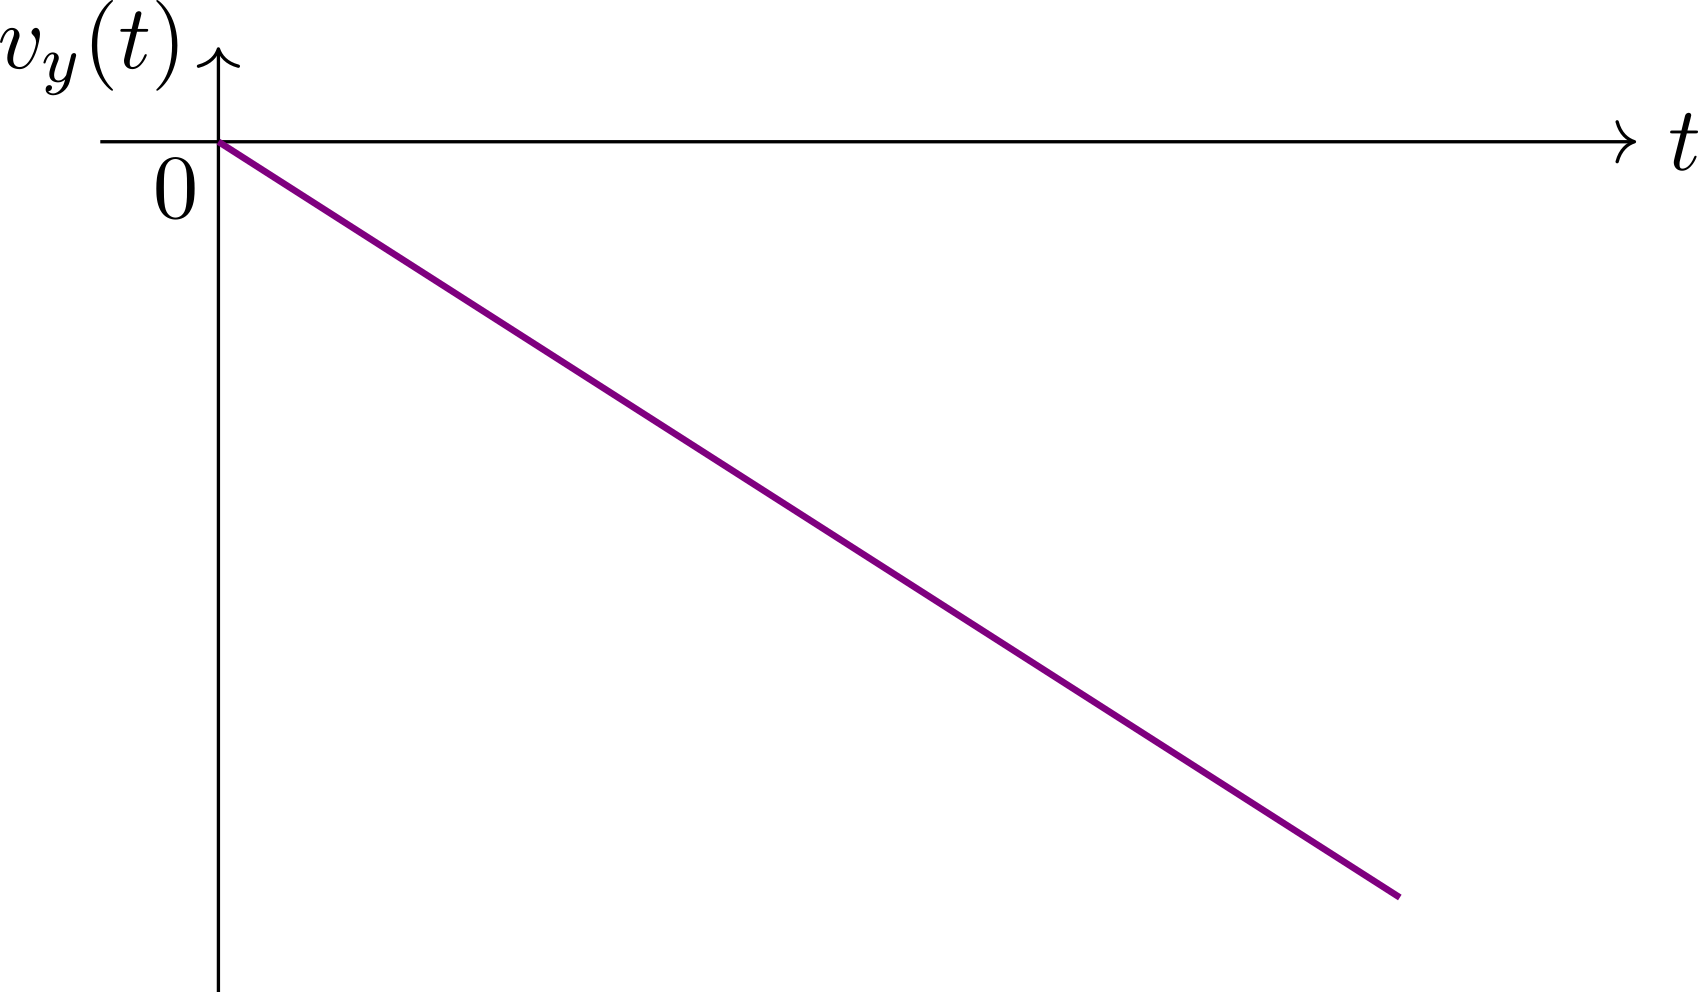
\includegraphics[width=6.5cm]{nov_vy}
	\end{center}
	\captionof{figure}{Évolution de $v_y$ avec le temps.}
\end{minipage}
\hfill
\begin{minipage}{0.45\linewidth}
	\begin{center}
		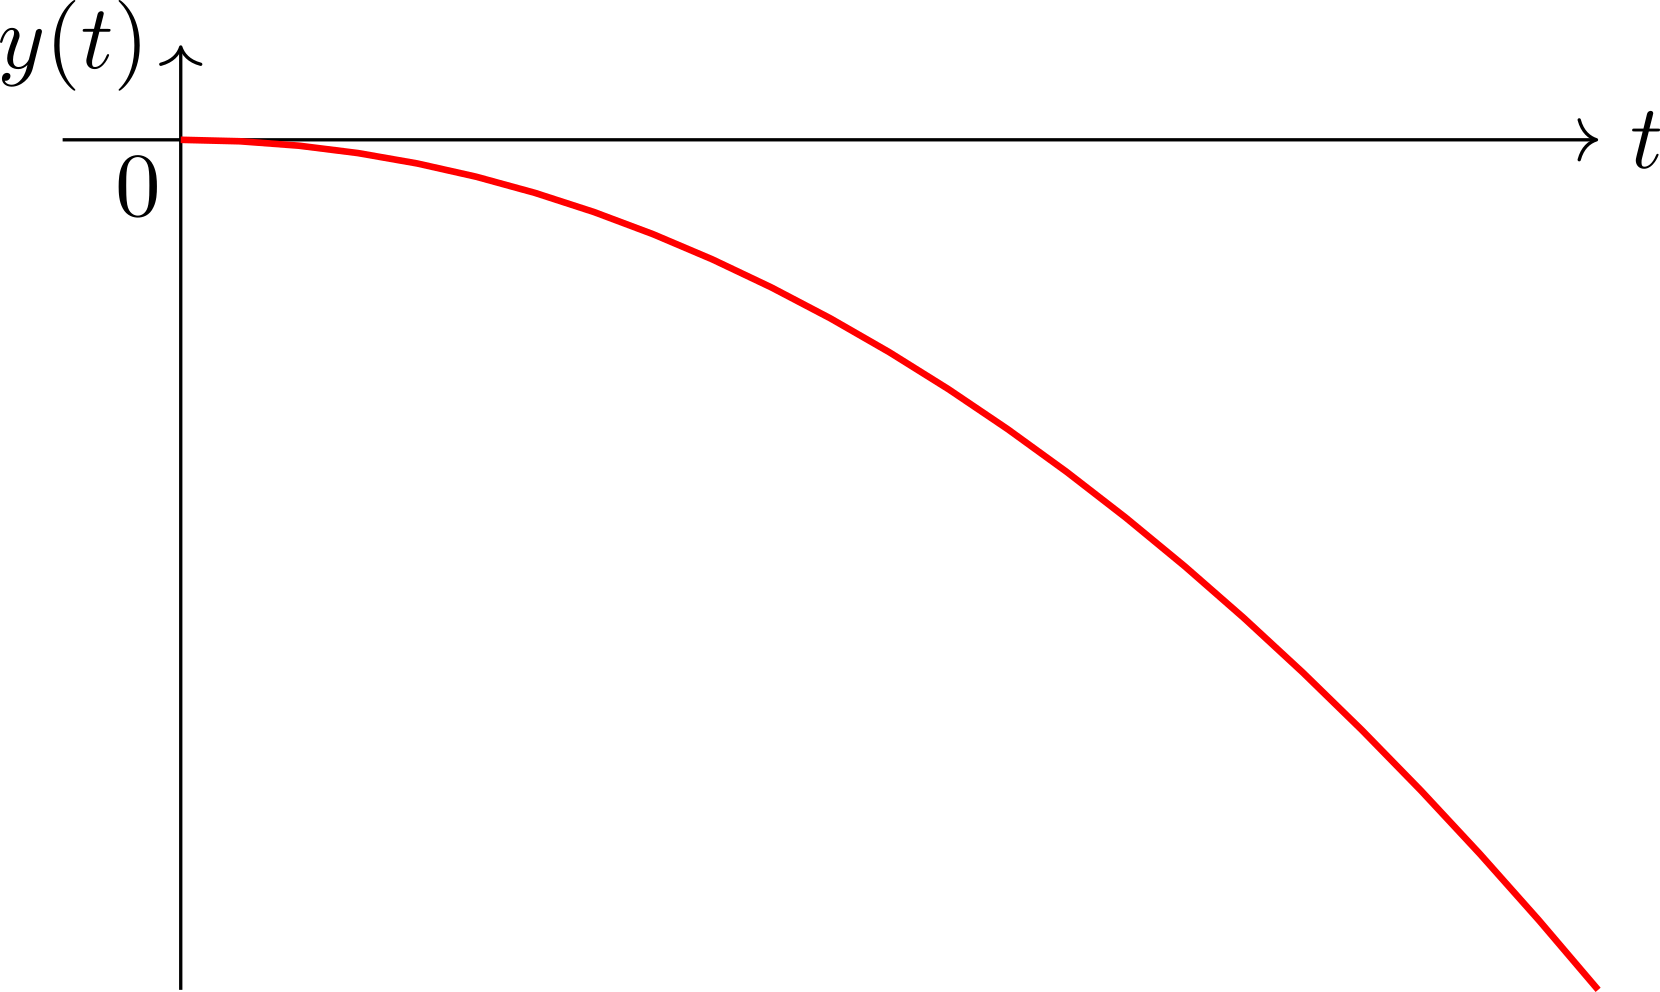
\includegraphics[width=6.5cm]{nov_y}
	\end{center}
	\captionof{figure}{Évolution de $y$ avec le temps.}
\end{minipage}
\hfill~

\subsection{Mouvement courbe uniformément accéléré}
\noindent
\begin{minipage}{0.70\linewidth}
	En reprenant la même situation que ci-dessus mais avec des conditions
	initiales non nulles, on trouvera un mouvement courbe. Prenons
	\[\vf(0) = v_0\ux\]
	avec $v_0 \neq 0$. On garde $\af = -g \uy$, le même repère et la même
	origine~: $\OM(0) = 0$. Par définition,
\end{minipage}
\hfill
\begin{minipage}{0.23\linewidth}
	\begin{center}
		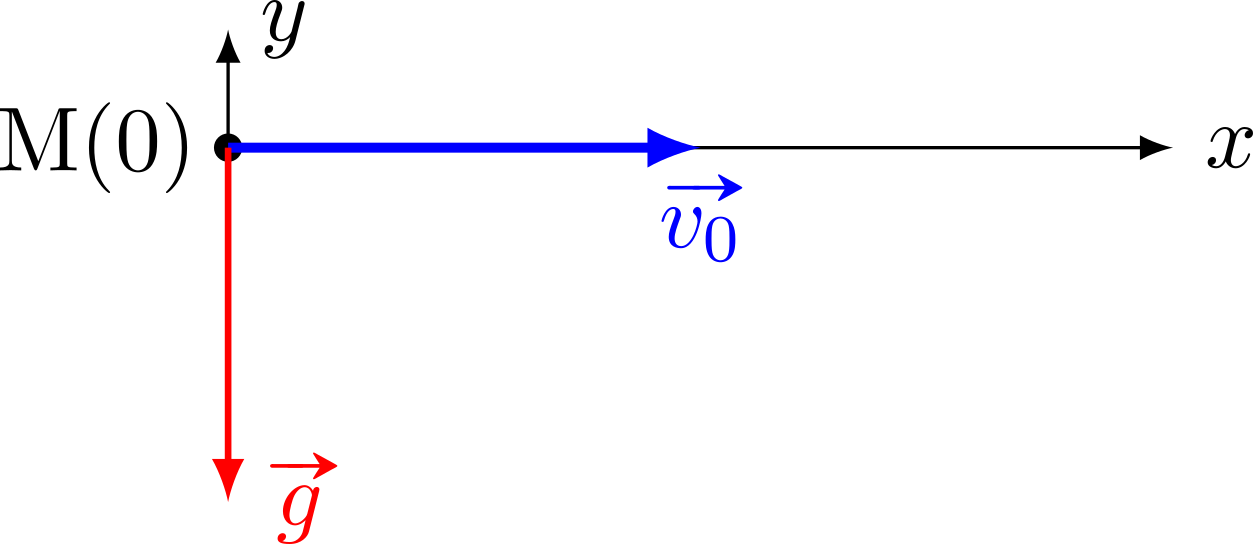
\includegraphics[width=\linewidth]{vo_init}
		\captionof{figure}{Situation initiale.}
	\end{center}
\end{minipage}

\[\psw{\af(t) = \xpp(t)\ux + \ypp(t)\uy + \zpp(t)\uz}\]
Soit
\[
	\psw{
		\left\{
		\begin{array}{l}
			\xpp(t) = 0  \\
			\ypp(t) = -g \\
			\zpp(t) = 0
		\end{array}
		\right.
		\Longrightarrow
		\left\{
		\begin{array}{l}
			\xp(t) = v_{x,0}       \\
			\yp(t) = -gt + v_{y,0} \\
			\zp(t) = v_{z,0}
		\end{array}
		\right.
	}\]
Or,
\[\psw{
		\vf(0) = v_0\ux
		\qdonc
		\left\{
		\begin{array}{l}
			\xp(0) = v_{x,0} = v_0 \\
			\yp(0) = v_{y,0} = 0   \\
			\zp(0) = v_{z,0} = 0
		\end{array}
		\right.
	}\]
Ainsi
\[
	\psw{
		\left\{
		\begin{array}{l}
			\xp(t) = v_0 \\
			\yp(t) = -gt \\
			\zp(t) = 0
		\end{array}
		\right.
		\Longrightarrow
		\left\{
		\begin{array}{l}
			x(t) = v_0t + x_{0}              \\
			y(t) = -\dfrac{1}{2}gt^2 + y_{0} \\
			z(t) = z_{0}
		\end{array}
		\right.
	}\]
Seulement,
\[\psw{
		\OM(0) = \of
		\qdonc
		\left\{
		\begin{array}{l}
			x(0) = y_{0} = 0 \\
			y(0) = y_{0} = 0 \\
			z(0) = z_{0} = 0
		\end{array}
		\right.
	}\]
Autrement dit,
\[\psw{
		\boxed{
			\left\{
			\begin{array}{l}
				x(t) = v_0t              \\
				y(t) = -\dfrac{1}{2}gt^2 \\
				z(t) = 0
			\end{array}
			\right.
		}}\]

\begin{minipage}{0.48\linewidth}
	\begin{center}
		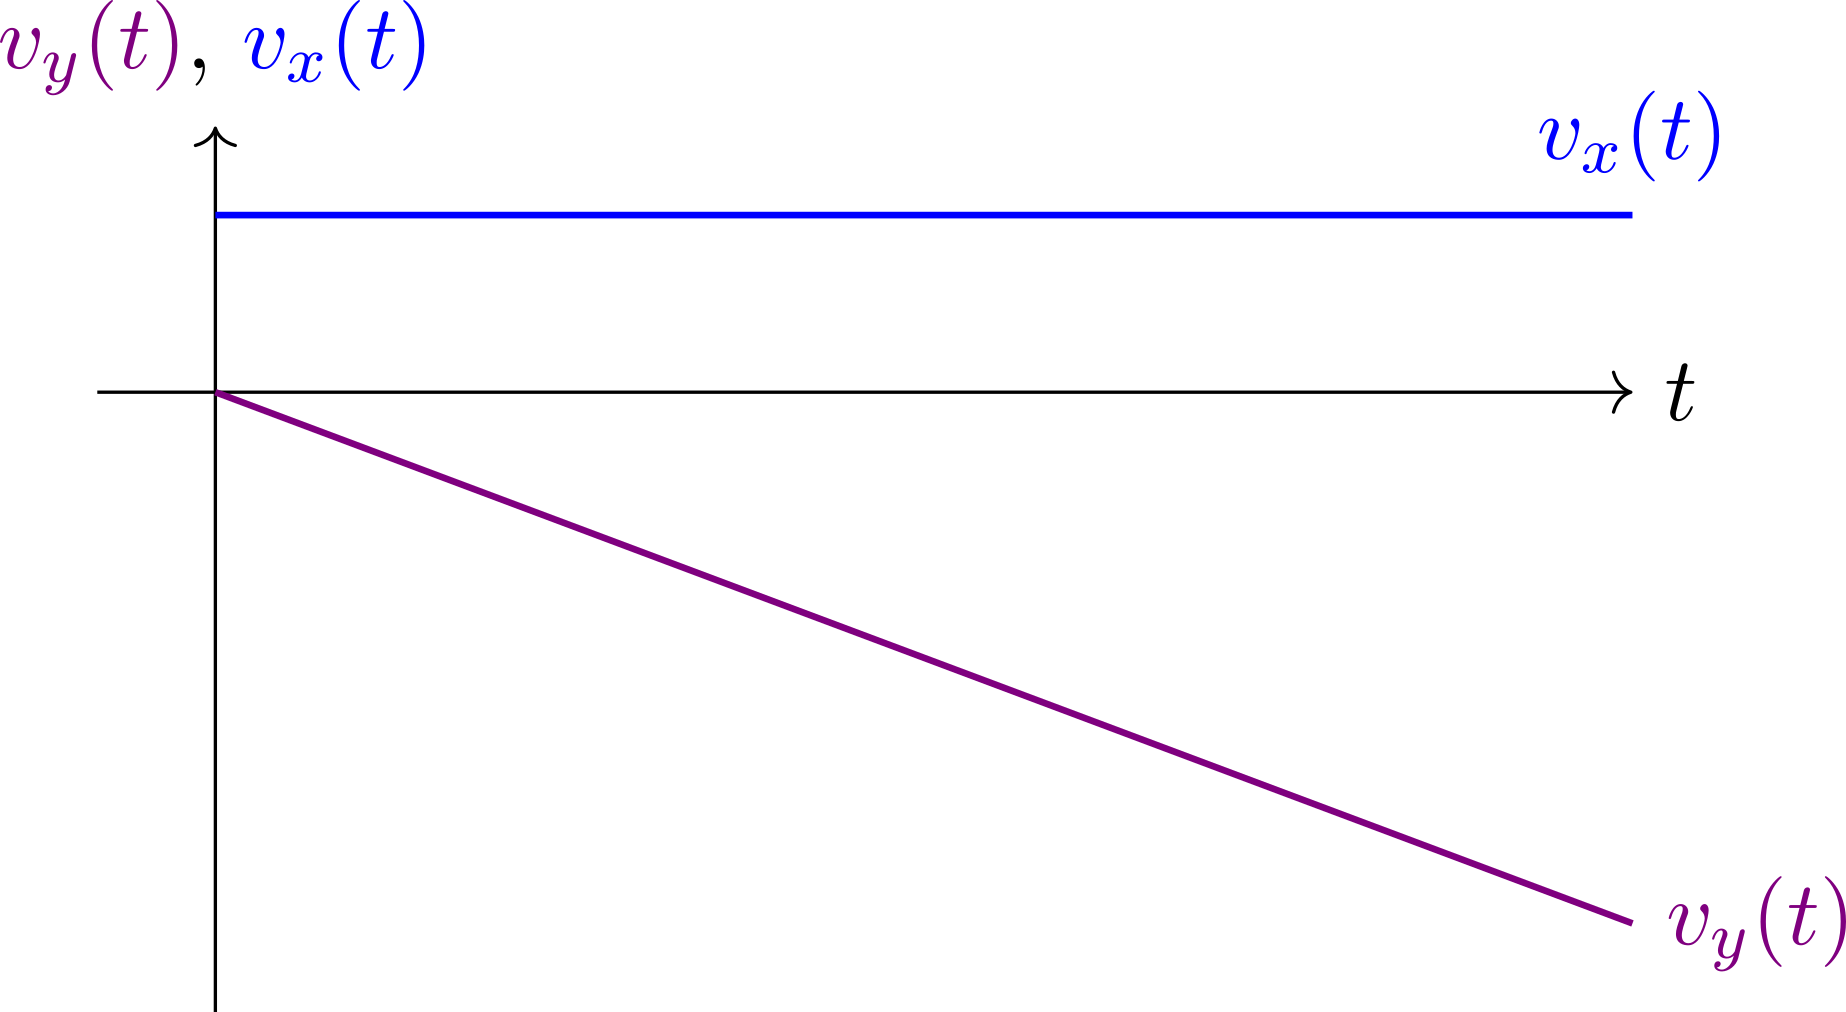
\includegraphics[width=\linewidth]{vo_vv}
	\end{center}
	\captionof{figure}{Évolution des vitesses avec le temps.}
\end{minipage}
\hfill
\begin{minipage}{0.48\linewidth}
	\begin{center}
		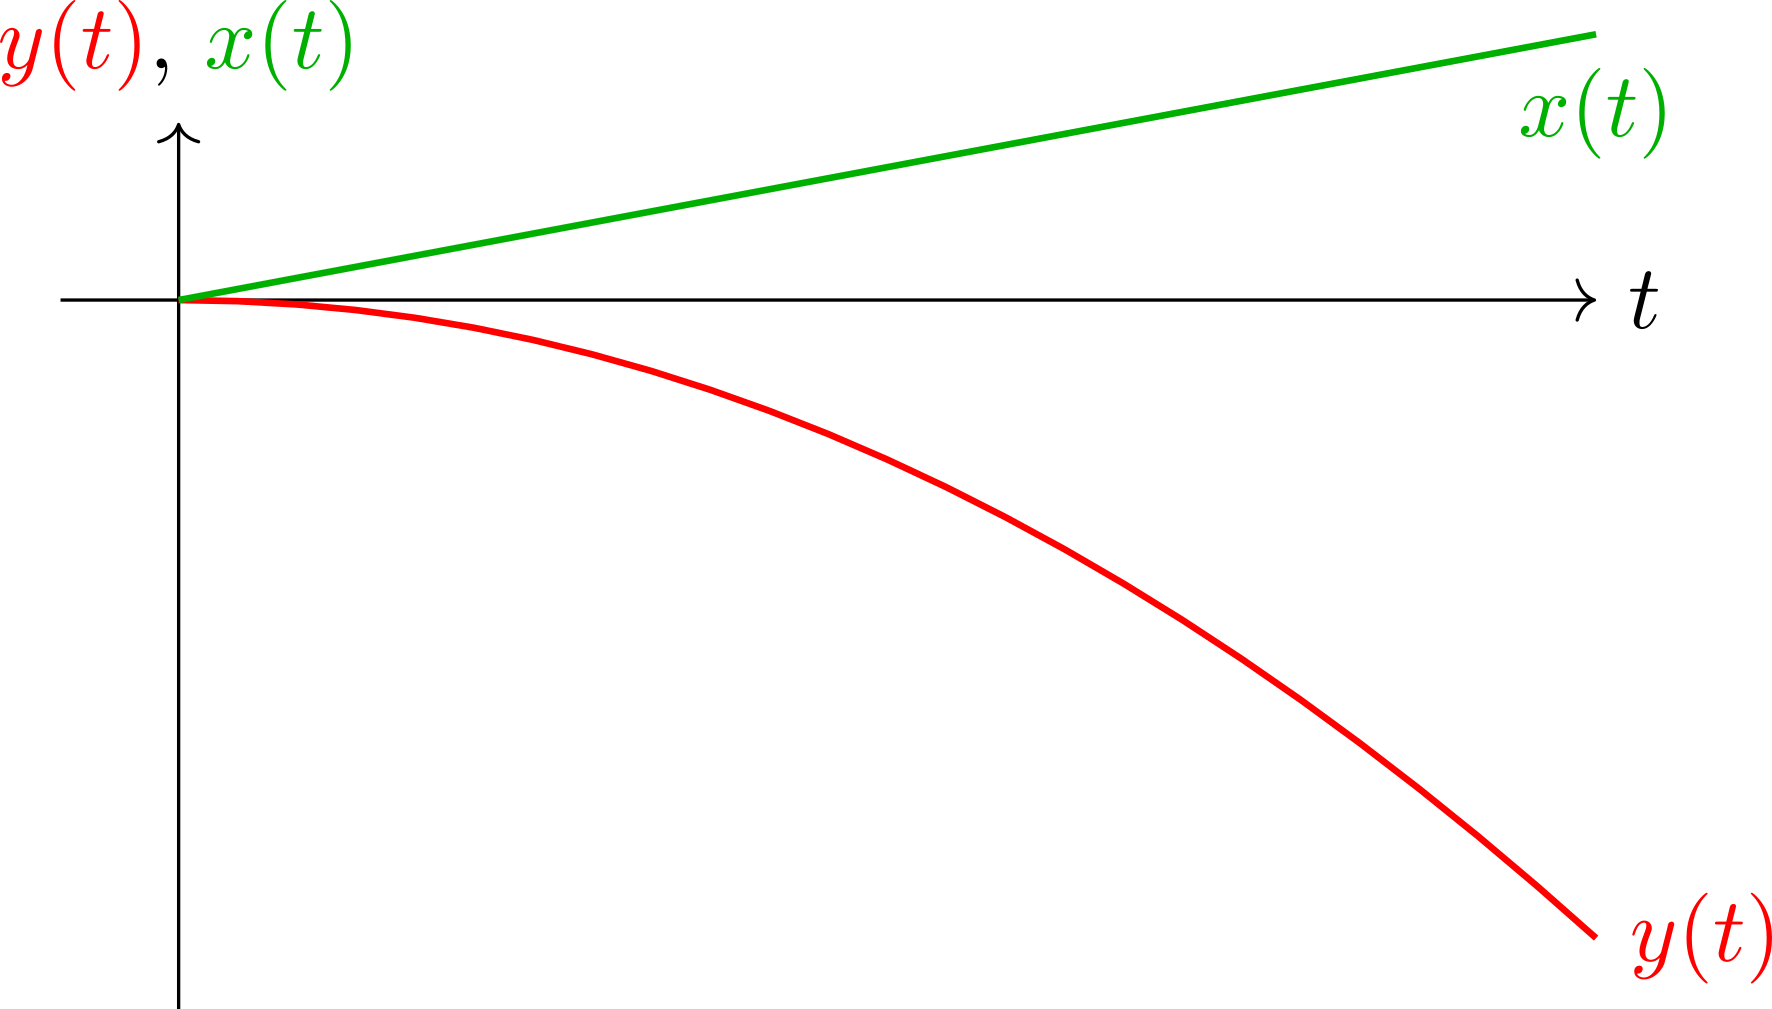
\includegraphics[width=\linewidth]{vo_xx}
	\end{center}
	\captionof{figure}{Évolution des positions avec le temps.}
\end{minipage} \bigbreak

\begin{minipage}{0.60\linewidth}
	Pour obtenir la trajectoire, on veut déterminer la courbe $y(x)$ décrite dans le
	plan $xy$. Pour cela, exprimons $t$ en fonction de $x$ et remplaçons $t$ dans
	l'expression de $y$~:
	\begin{gather*}
		t = \frac{x}{v_0}\\
		\Rightarrow
		y(x) = - \frac{1}{2}g \left( \frac{x}{v_0} \right)^2
		\Leftrightarrow
		\boxed{y(x) = - \frac{g}{2v_0{}^2}x^2}
	\end{gather*}
	La trajectoire obtenue est alors une parabole.
\end{minipage}
\hfill
\begin{minipage}{0.35\linewidth}
	\begin{center}
		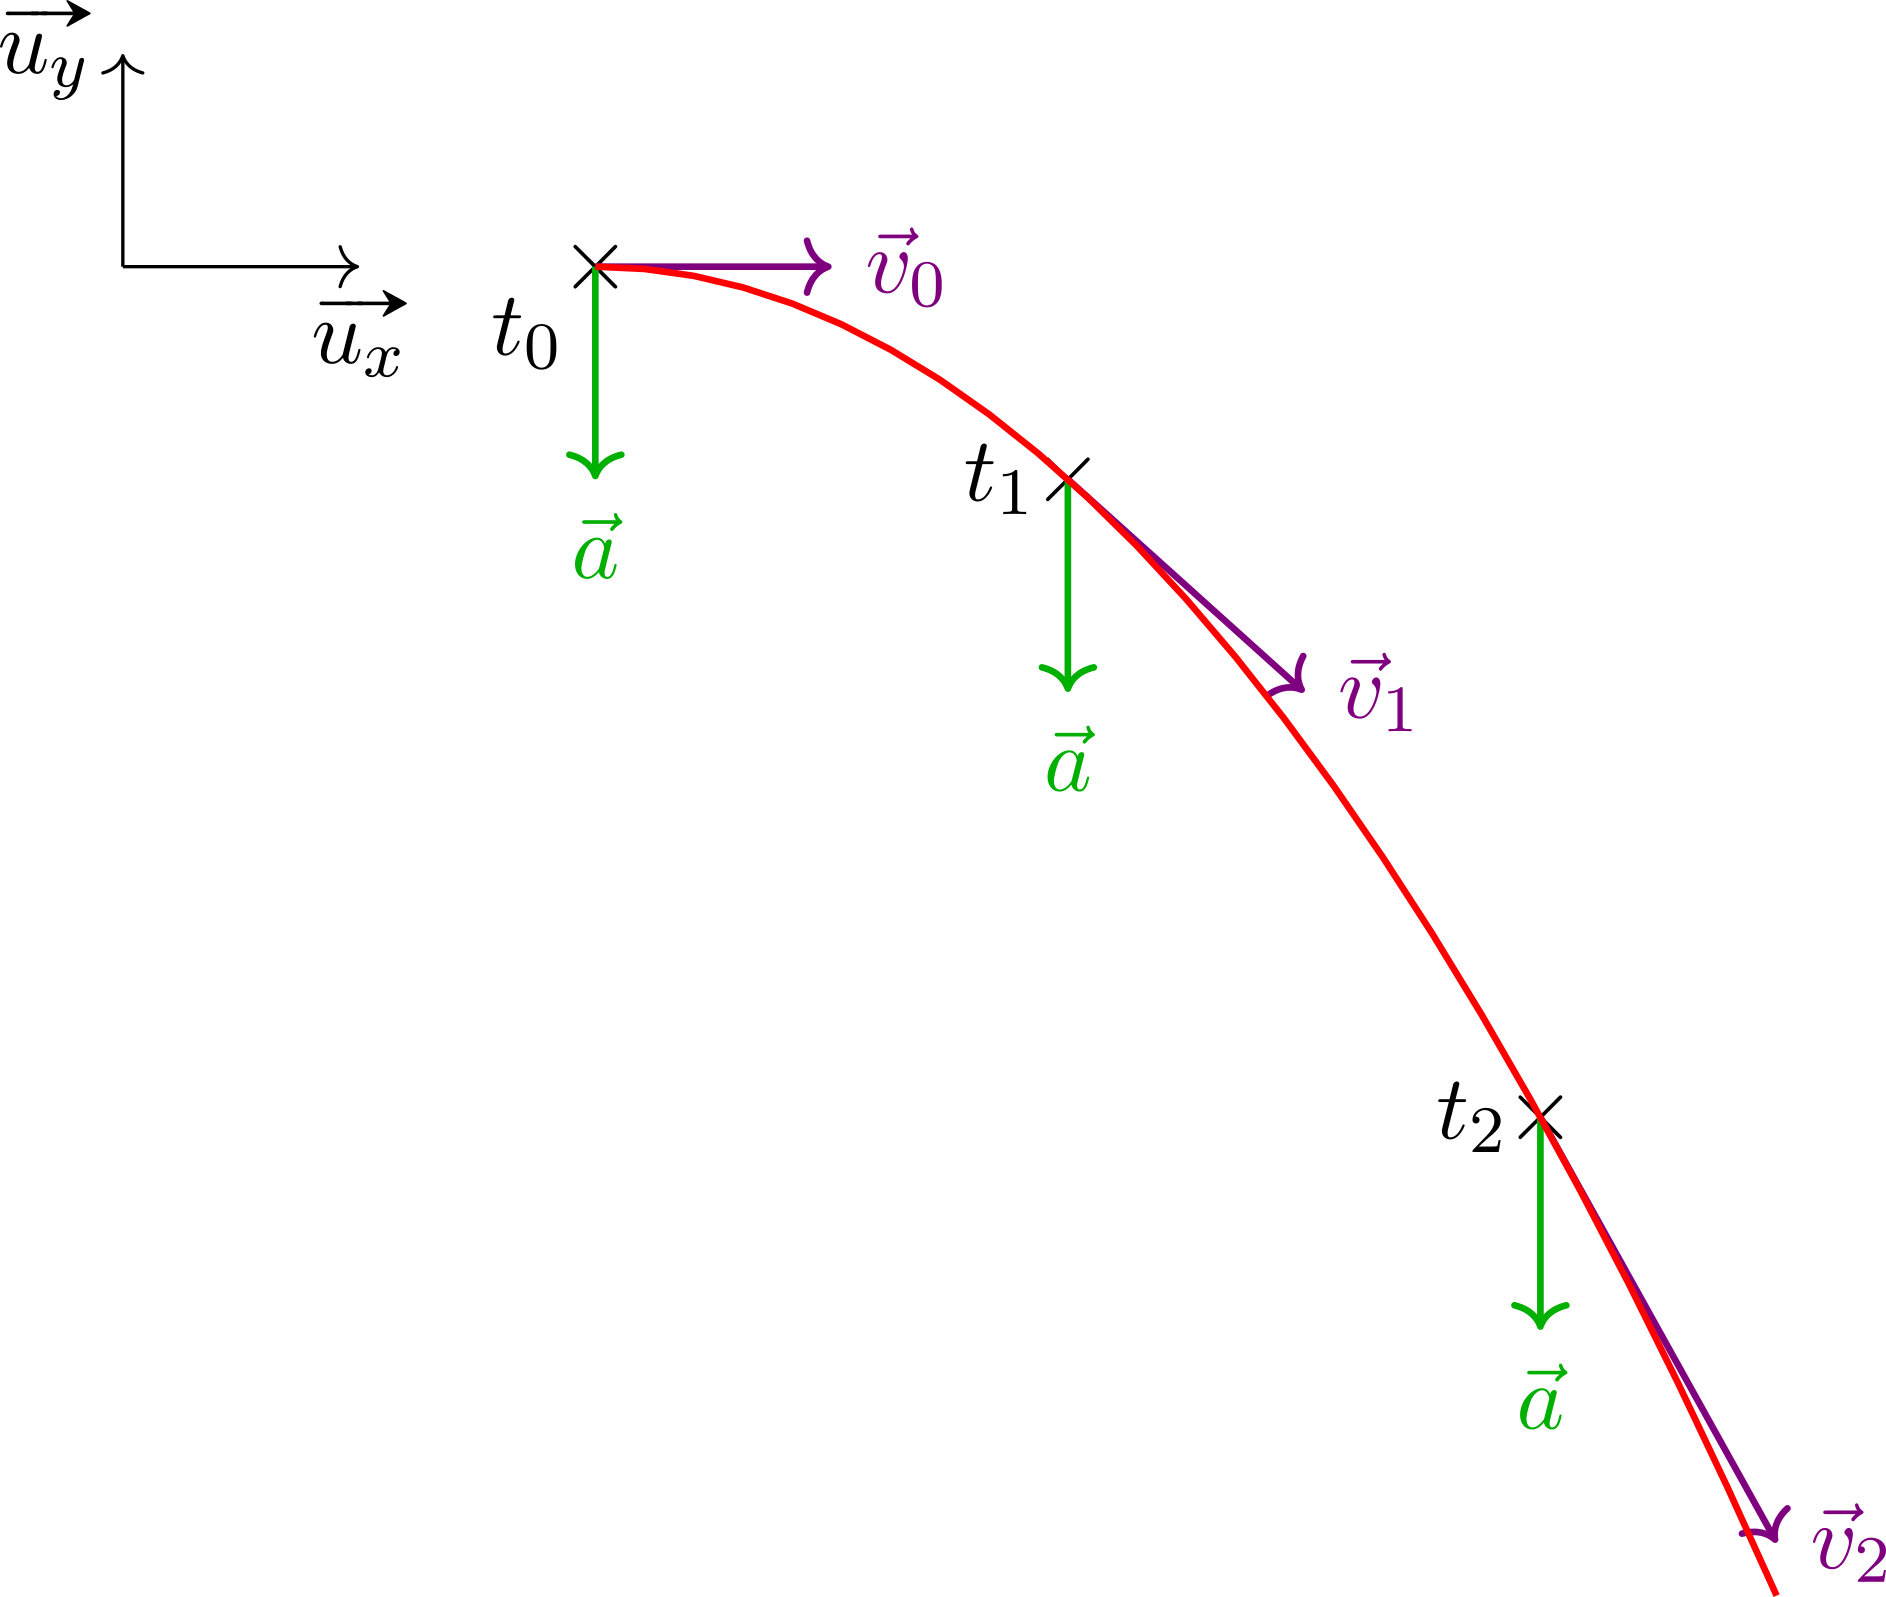
\includegraphics[width=\linewidth]{vo_traj}
		\captionof{figure}{Trajectoire parabolique.}
	\end{center}
\end{minipage}

\end{document}
